
\phantomsection 
\section{User Flows}
This section of the document covers the user flows regarding most of the use cases. The user flows are divided by actor and for each user flow is specified which related use cases are implemented.
In order to simplify user flows and ease understanding, some general flows such as "Fill Form" were created. Such flows are described at the beginning of the document, shown entirely within the first user flow that makes use of them and then simply referred to in the rest of the user flows. Moreover - in the user flows covering multiple use cases - the use case that a particular branch covers is written in the transition arrow.

\phantomsection 
\subsection{Diagram Legend}
The User Flows make use of different shapes and colors, each with an associated meaning. In particular:
\begin{itemize}
    \item \textbf{Light blue Ellipse: }Used to represent the start, end or stop of the User Flows, "Start" refers to the beginning of the flow, "End" to the successful completion of the user flow (i.e. the end of the happy path) and "Stop" refers to the unsuccessful end of the flow, caused by some error. Moreover "Continue" is used in general flows to specify where the next step of a User Flow including a general flow will be.
    \item \textbf{Green Rounded Rectangle: }Used to represent the states of the interface (i.e. what an actor sees at some point in the flow).
    \item \textbf{Yellow Diamond: }Used to represent the decisions in the User Flows and the choice of page from the Navbar.
    \item \textbf{Red Rounded Rectangle: }Used to represent the actions in the User Flows.
    \item \textbf{Pink Rounded Rectangle: }Used to represent general flows (e.g., "Fill Form"), which are described in detail at the beginning of the document. When inserting a general flow into a larger diagram, the following logic applies:
        \begin{enumerate}
            \item The pink rounded rectangle must be preceded by an interface state (e.g., "Registration Form").
            \item This interface state represents the first step of the general flow.
            \item The step immediately following the general flow replaces the "Continue" lightblue ellipse from the base diagram.
        \end{enumerate}
\end{itemize}

\newpage
\phantomsection 
\subsection{Actors}
The actors are:
\begin{itemize}
    \item \textbf{User:} This actor represents a general user who could be a Patient, Doctor, Head of Hospital or Head of Department. A User's main functionalities cover registration, login, calendar view and profile management.
    \item \textbf{Admin:} This actor represents the system administrator, whose main activities cover the management of the hospital structure.
    \item \textbf{Patient:} This actor represents a patient within the healthcare system, whose main functionalities regard the booking and management of appointments.
    \item \textbf{Doctor:} This actor represents a general doctor within a healthcare system, including Head of Hospital and Head of Department. A Doctor's main functionalities regard the management and tracking of examinations and the consultations of Patients' medical records.
    \item \textbf{Head of Hospital:} This actor represents a specific doctor who was appointed as the head of a hospital, whose main functionalities regard the management of a hospital facility
    \item \textbf{Head of Department:} This actor represents a specific doctor who was appointed as the head of a department, whose main functionalities regard the management of a department within a hospital facility.
\end{itemize}
% --- eg ---
\newpage
\begin{minipage}{\textwidth}
    \phantomsection 
    \subsection{General Flow - Fill Form Flow}
    The following diagram describes in detail the steps of the general Fill Form flow, expanded in the user flow  \hyperref[UF12]{UF12. Patient - Registration and Validation}.
    
    \begin{center}
        
\includegraphics[width=8cm]{User_Flows/FillForm.png}
        \captionof{figure}{General Fill Form Flow}
    \end{center}
    %\begin{itemize}   
    %\end{itemize}
\end{minipage}
\vspace{3em}

\begin{minipage}{\textwidth}
    \phantomsection 
    \subsection{General Flow - Detailed Access Flow}
    The following diagram describes in detail the steps of the general Detailed Access flow, expanded in the user flow \hyperref[UF16]{UF16. Patient - Medical Record and Prescriptions consultation}.
    
    \begin{center}
        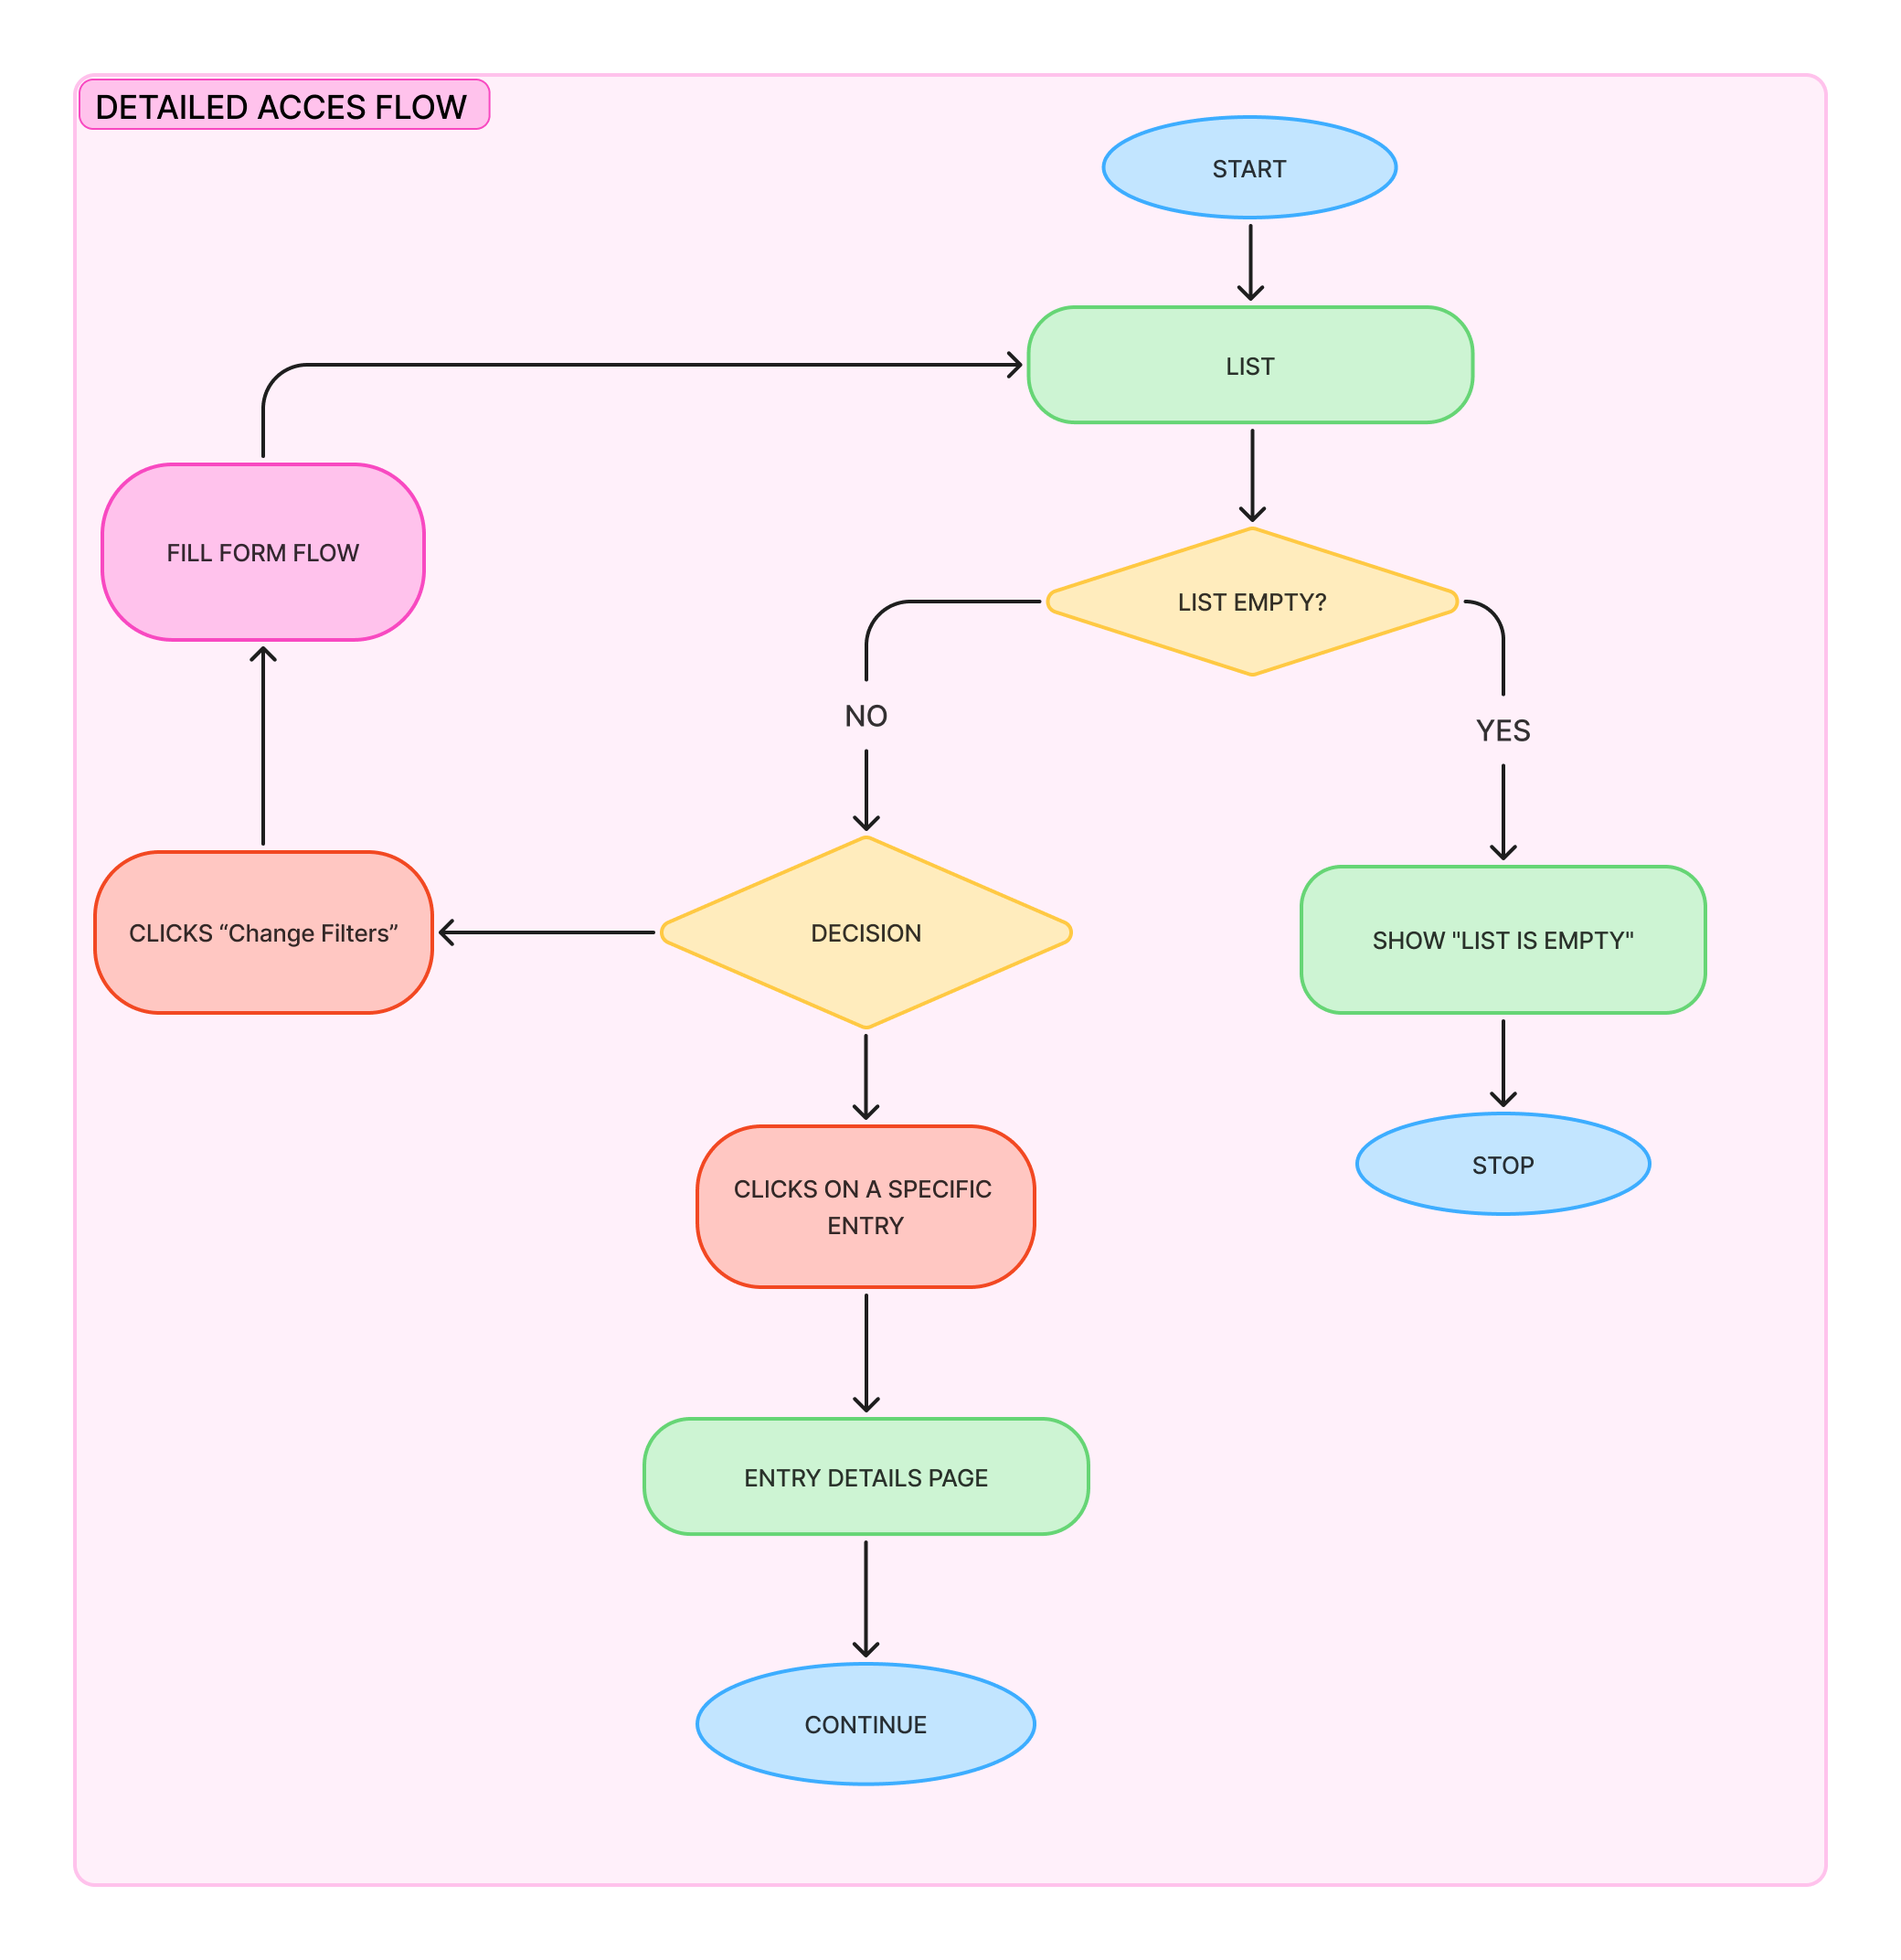
\includegraphics[width=9cm]{User_Flows/DetailedAccess.png}
        \captionof{figure}{General Detailed Access Flow}
    \end{center}
    %\begin{itemize}   
    %\end{itemize}
\end{minipage}
\vspace{3em}

\begin{minipage}{\textwidth}
    \phantomsection 
    \subsection{General Flow - Creation Flow}
    The following diagram describes in detail the steps of the general Creation flow, expanded in the user flow \hyperref[UF6]{UF6. Admin - Create Insurance Policy, Hospital, Treatment, Department. Register Doctor}.
    
    \begin{center}
        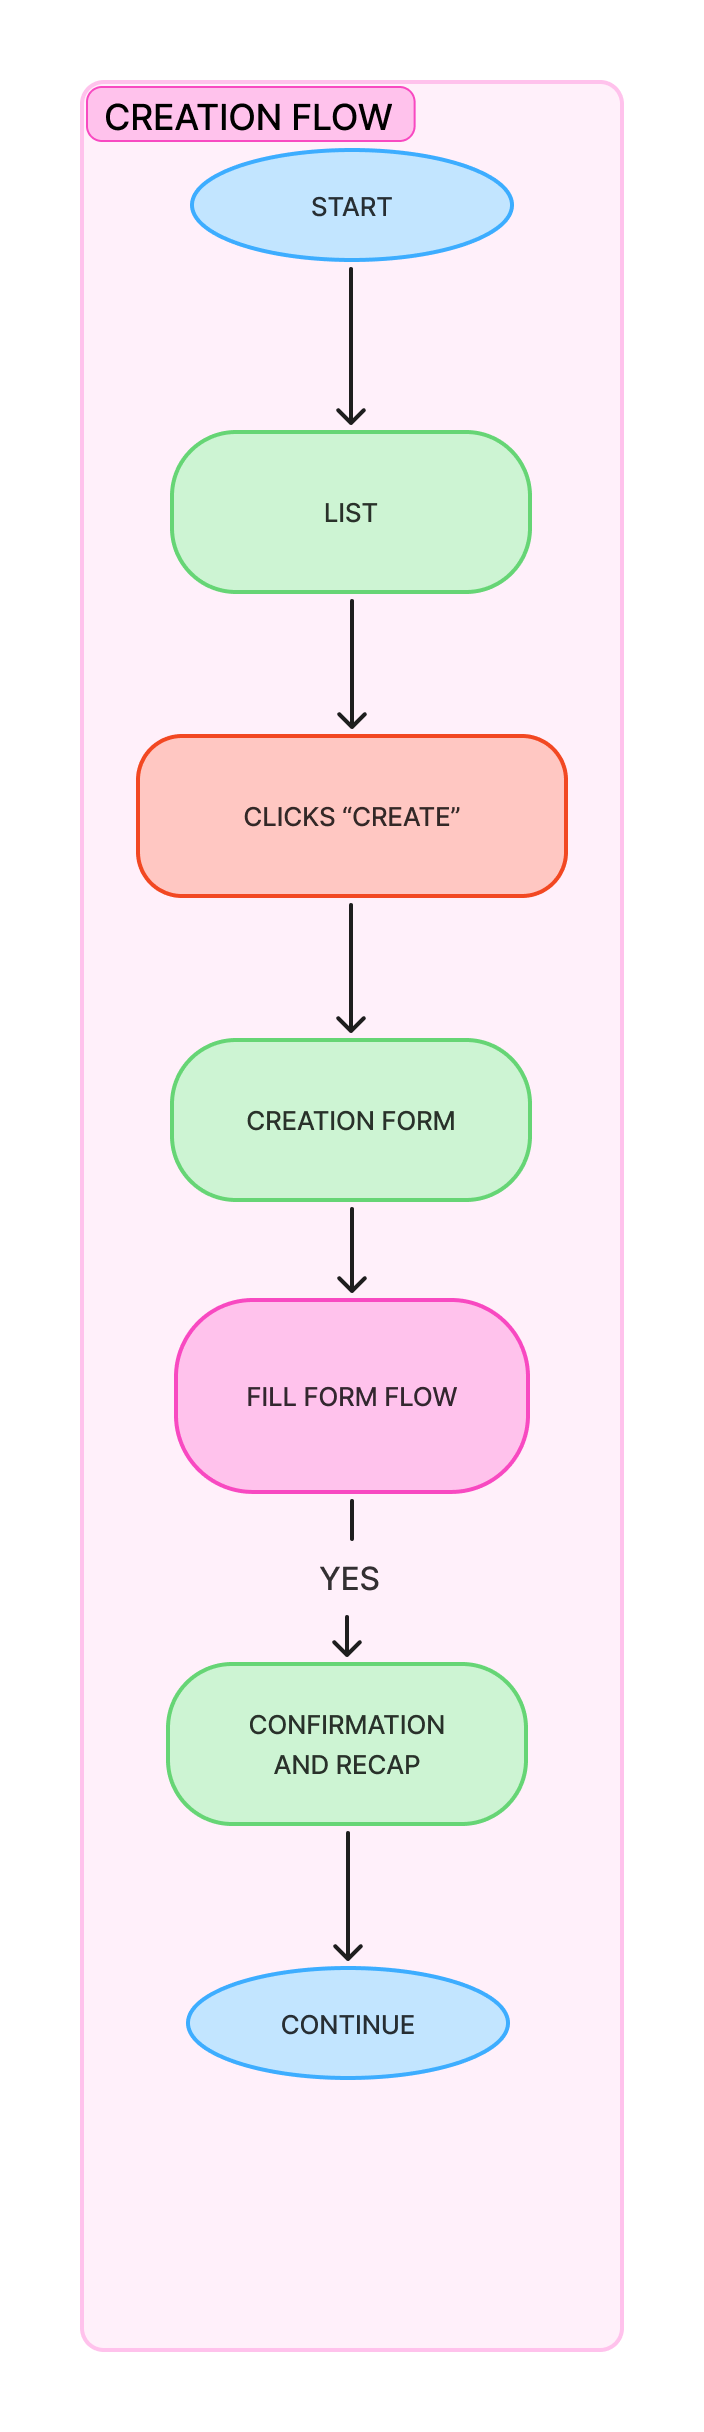
\includegraphics[width=5cm]{User_Flows/Creation.png}
        \captionof{figure}{General Creation Flow}
    \end{center}
    %\begin{itemize}   
    %\end{itemize}
\end{minipage}
\vspace{3em}

\begin{minipage}{\textwidth}
    \phantomsection
    \subsection{General Flow - Edit Flow}
    The following diagram describes in detail the steps of the general Edit flow, expanded in the user flow \hyperref[UF7]{UF7. Admin - Edit Insurance Policy, Hospital, Treatment, Department. Register Doctor}.
    \begin{center}
        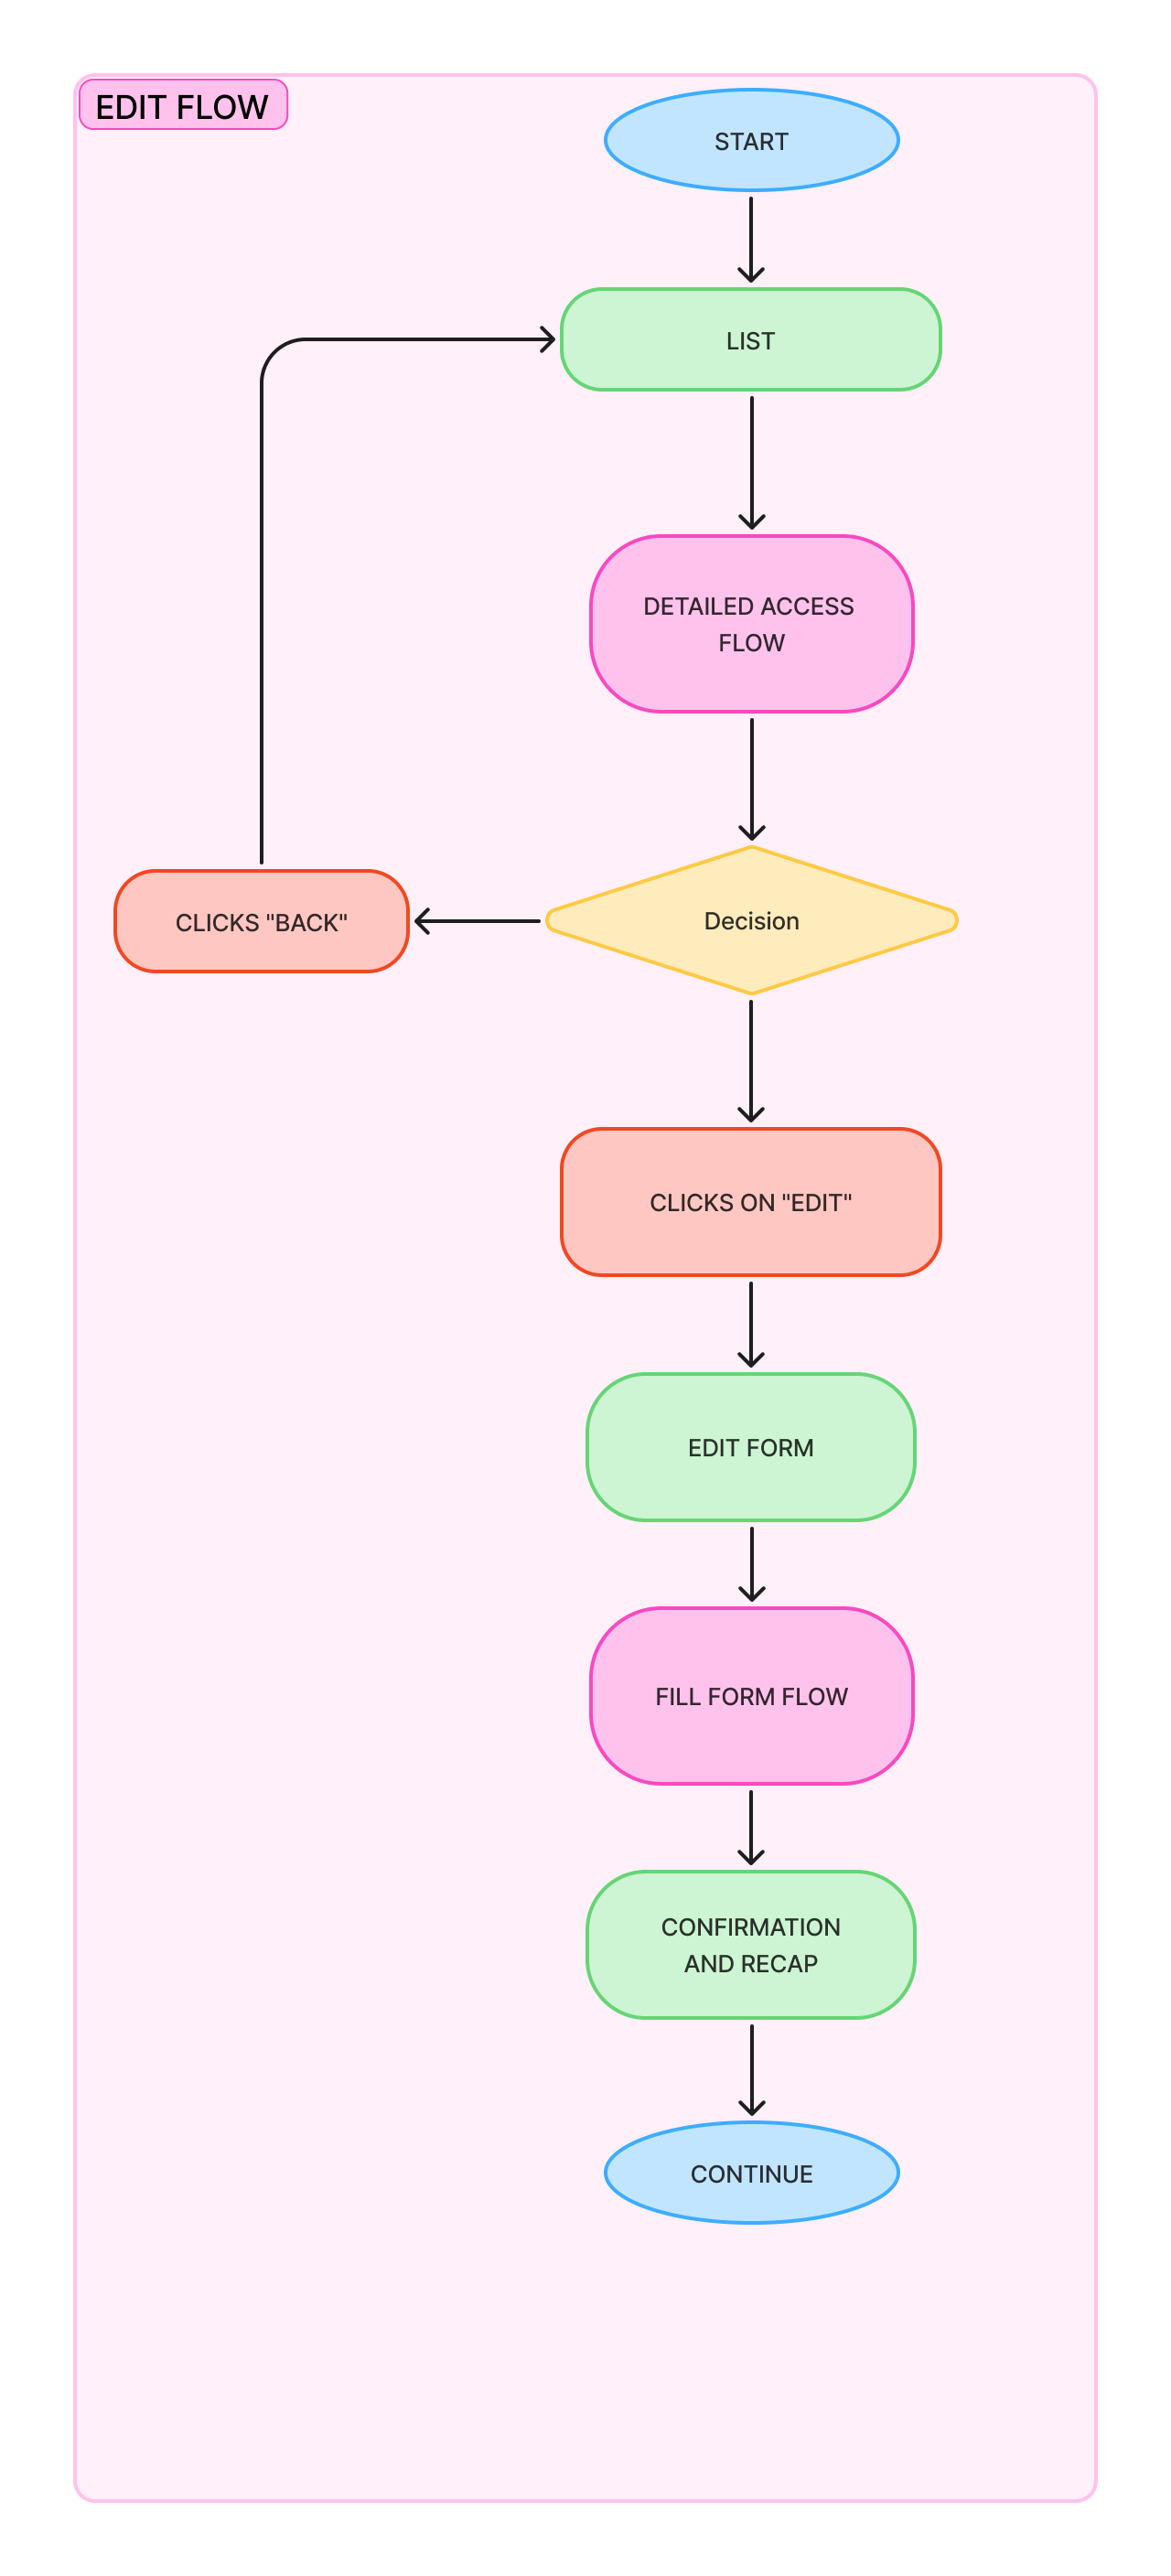
\includegraphics[width=8cm]{User_Flows/Edit.png}
        \captionof{figure}{General Edit Flow}
    \end{center}
    %\begin{itemize}   
    %\end{itemize}
\end{minipage}
\vspace{3em}

\begin{minipage}{\textwidth}
    \phantomsection
    \subsection{General Flow - Deletion Flow}
    The following diagram describes in detail the steps of the general Deletion flow, expanded in the user flow \hyperref[UF8]{UF8. Admin - Deactivate Insurance Policy, Hospital, Treatment, Department}.
    
    \begin{center}
        
\includegraphics[width=8cm]{User_Flows/Deletion.png}
        \captionof{figure}{General Deletion Flow}
    \end{center}
    %\begin{itemize}   
    %\end{itemize}
\end{minipage}
\vspace{3em}

\begin{minipage}{\textwidth}
    \phantomsection
    \subsection{UF1. User - Login and Recovery}
    The following user flow shows the process of User login and account recovery. UC24 is implemented with mock IDP login, while UC26 is not implemented.
    It refers to use cases \textbf{UC24, UC26}, and methods \textbf{login(credentials), requestPasswordReset()} from the class \textbf{User} of the class diagram.
    
    \begin{center}
        
\includegraphics[width=0.8\textwidth]{User_Flows/LoginRecovery.png}
        \captionof{figure}{User flow regarding User Login and Recovery}
    \end{center}
    %\begin{itemize}   
    %\end{itemize}
\end{minipage}
\vspace{3em}


\begin{minipage}{\textwidth}
    \phantomsection
    \subsection{UF2. User - Internal Calendar}
    The following user flow shows the steps a user takes to view their calendar and see the details of a booked appointment. UC28, UC38 are implemented.
    It refers to use cases \textbf{UC30, UC28}, and methods \textbf{Calendar.getAppointments(), Appointment.getDetails()} from the class \textbf{Calendar, Appointment} of the class diagram.
    
    \begin{center}
        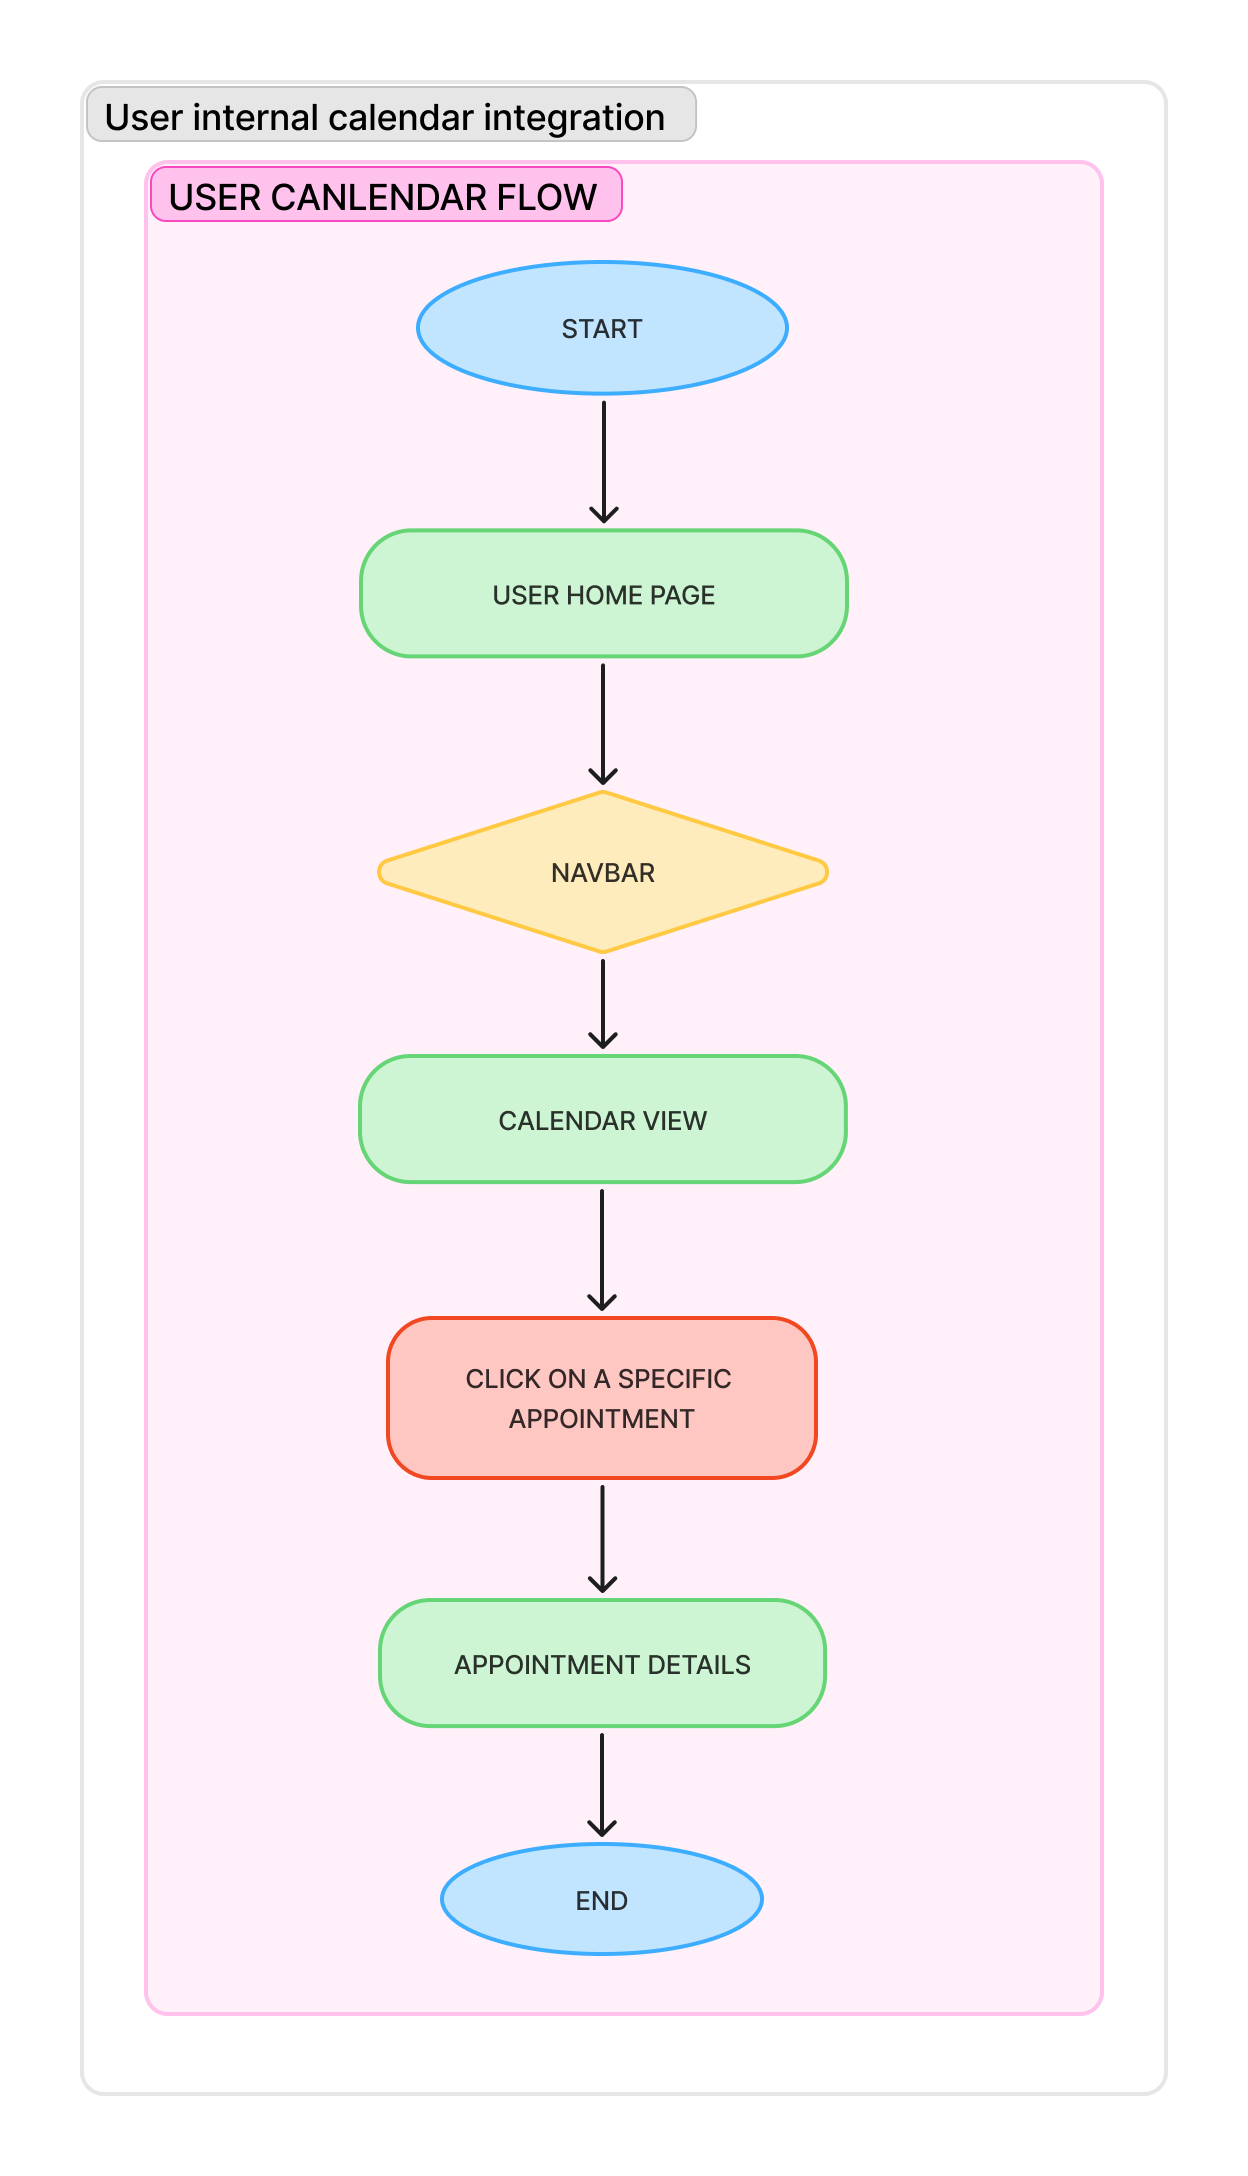
\includegraphics[width=8cm]{User_Flows/UserInternalCalendar.png}
        \captionof{figure}{User flow regarding Internal Calendar integration and View Appointment Details}
    \end{center}
    %\begin{itemize}   
    %\end{itemize}
\end{minipage}
\vspace{3em}


\begin{minipage}{\textwidth}
    \phantomsection
    \subsection{UF3. User - Profile Update and Deletion}
    The following user flow shows the steps a user takes to update and delete their profile. UC7 is implemented, UC41 is partially implemented as the deletion of the account occurs immediately rather than after 30 days.
    It refers to use cases \textbf{UC7, UC41}, and methods \textbf{viewProfile(), updateProfile(newData), deleteAccount()} from the class \textbf{User} of the class diagram.
    
    \begin{center}
        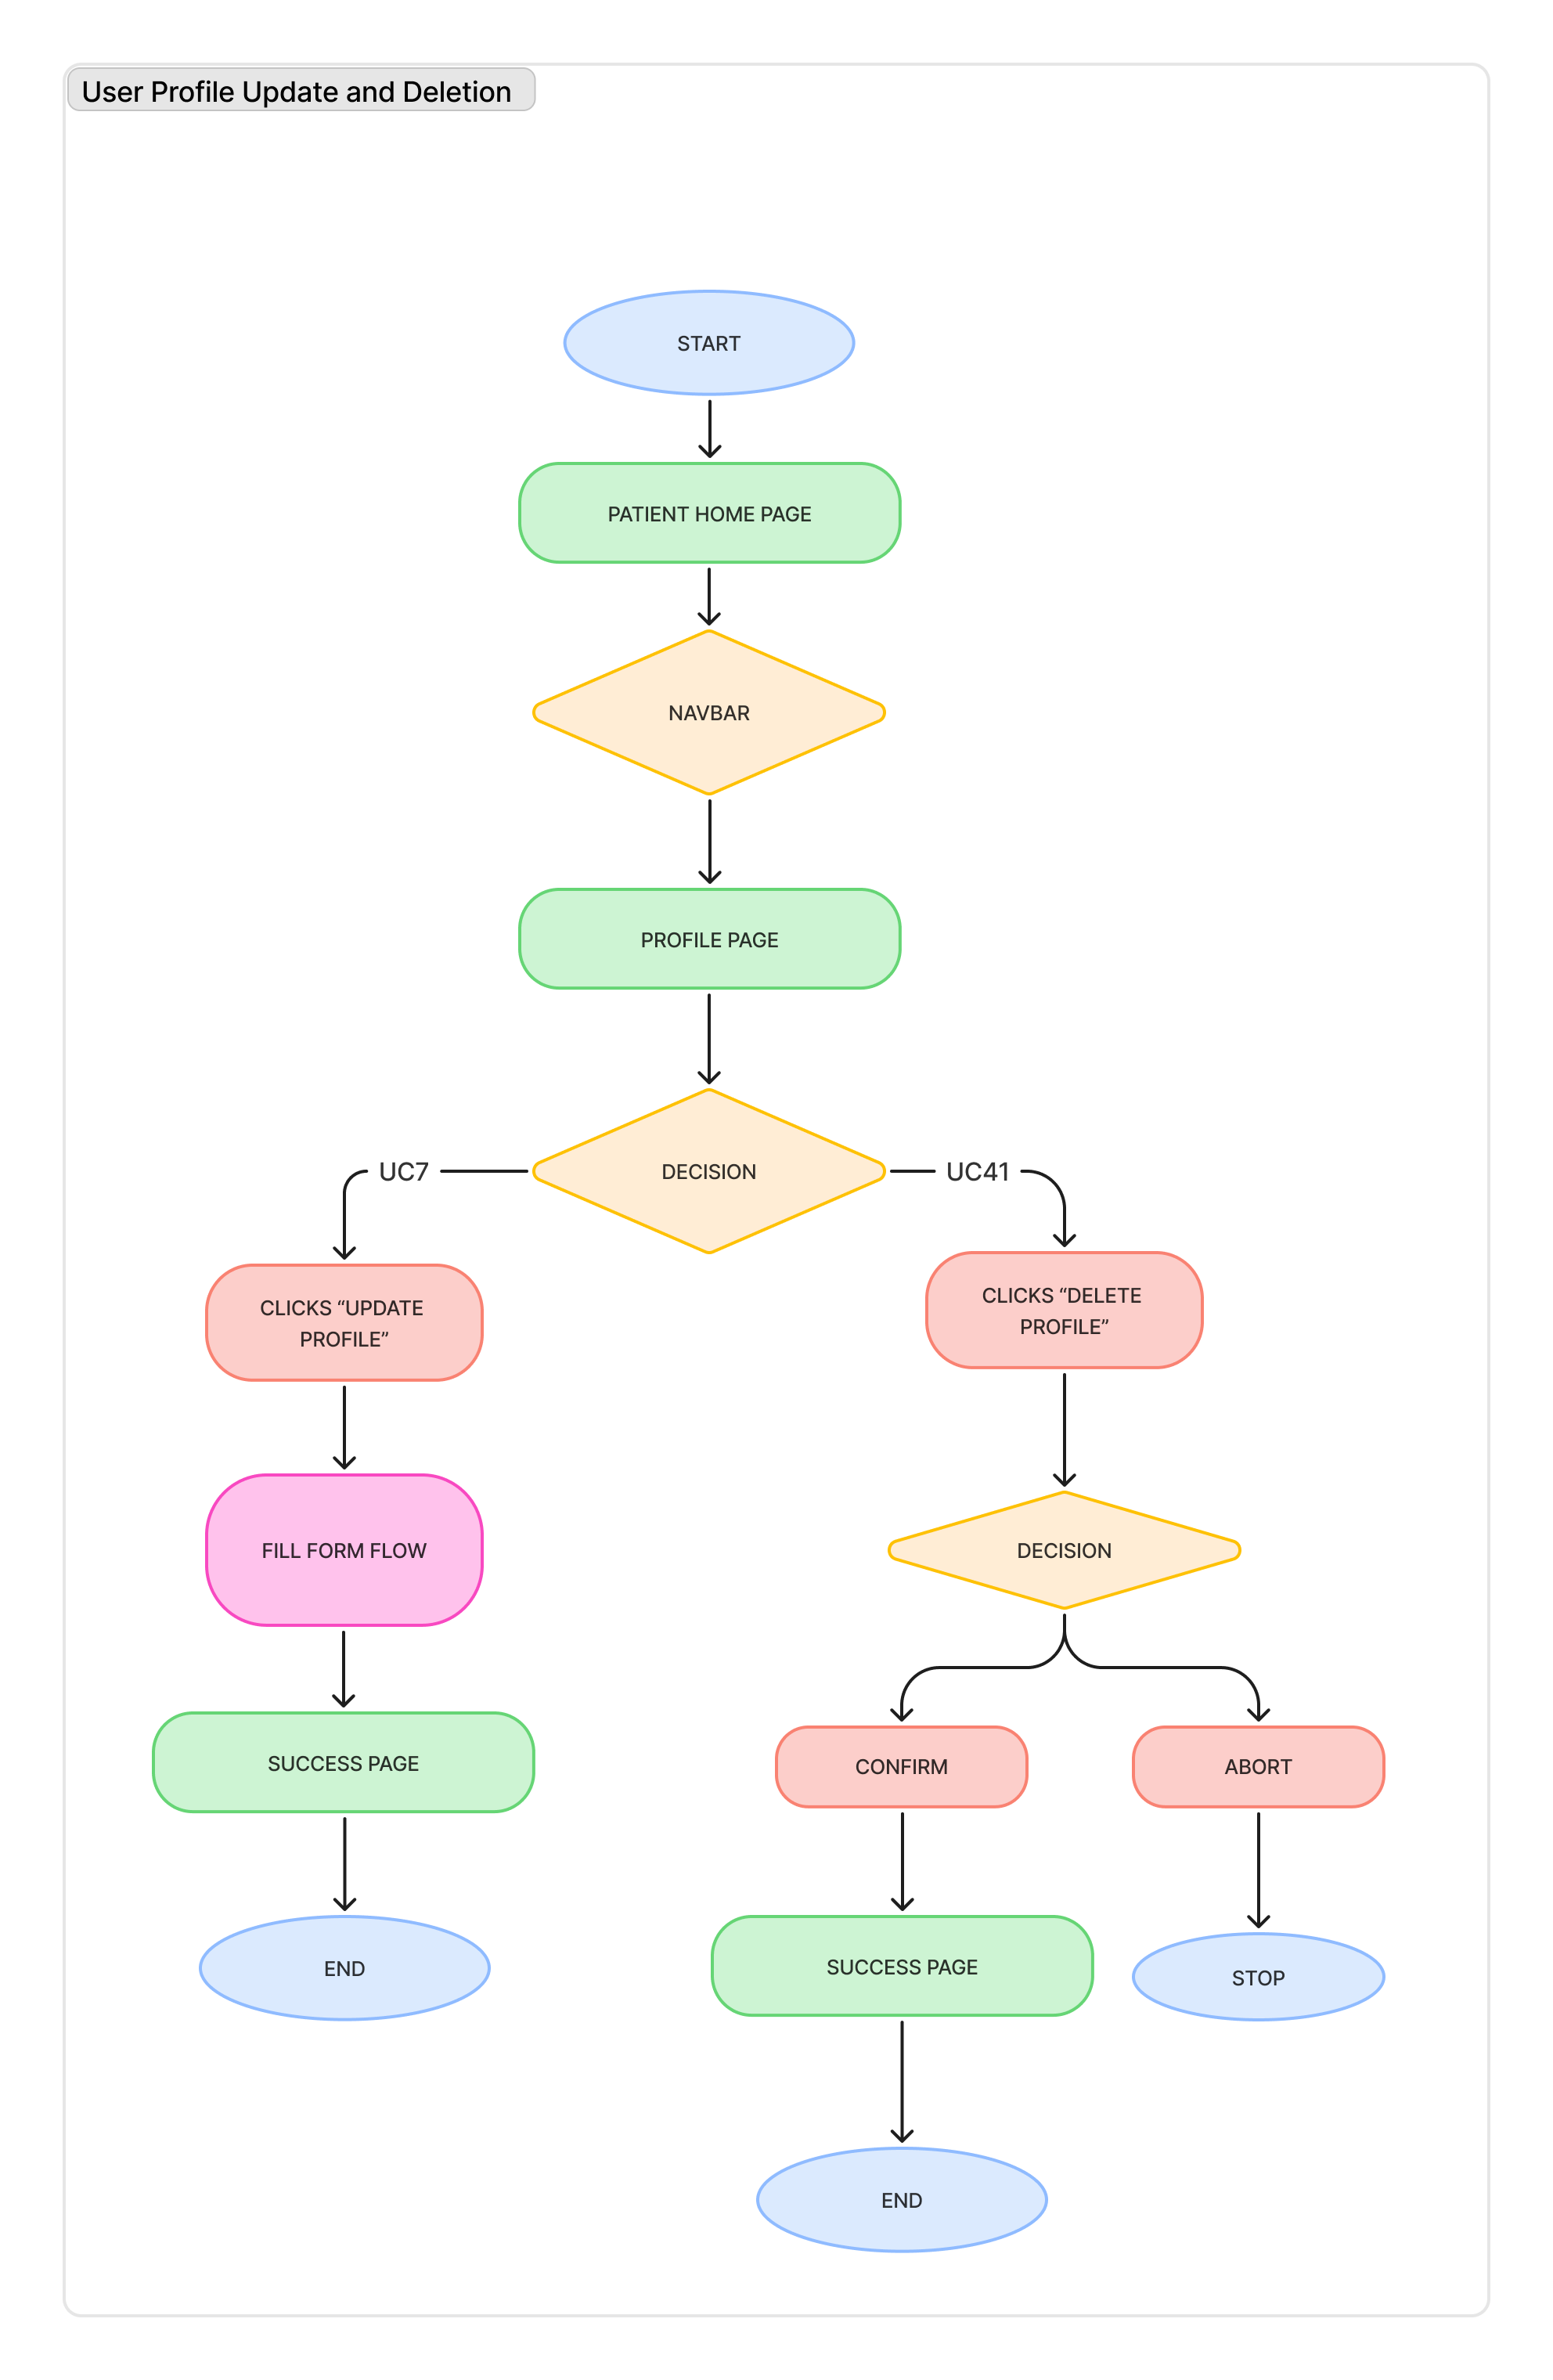
\includegraphics[width=0.8\textwidth]{User_Flows/ProfileUpdateDeletion.png}
        \captionof{figure}{User flow regarding Profile Update and Account Deletion}
    \end{center}
    %\begin{itemize}   
    %\end{itemize}
\end{minipage}
\vspace{3em}

\begin{minipage}{\textwidth}
    \phantomsection
    \subsection{UF4. User - Export Calendar}
    The following user flow shows the steps a user takes to export their appointment to an external calendar. UC31 is not implemented.
    It refers to use case \textbf{UC31}, and methods \textbf{generateExportToken()} from the class \textbf{Calendar} of the class diagram.
    
    \begin{center}
        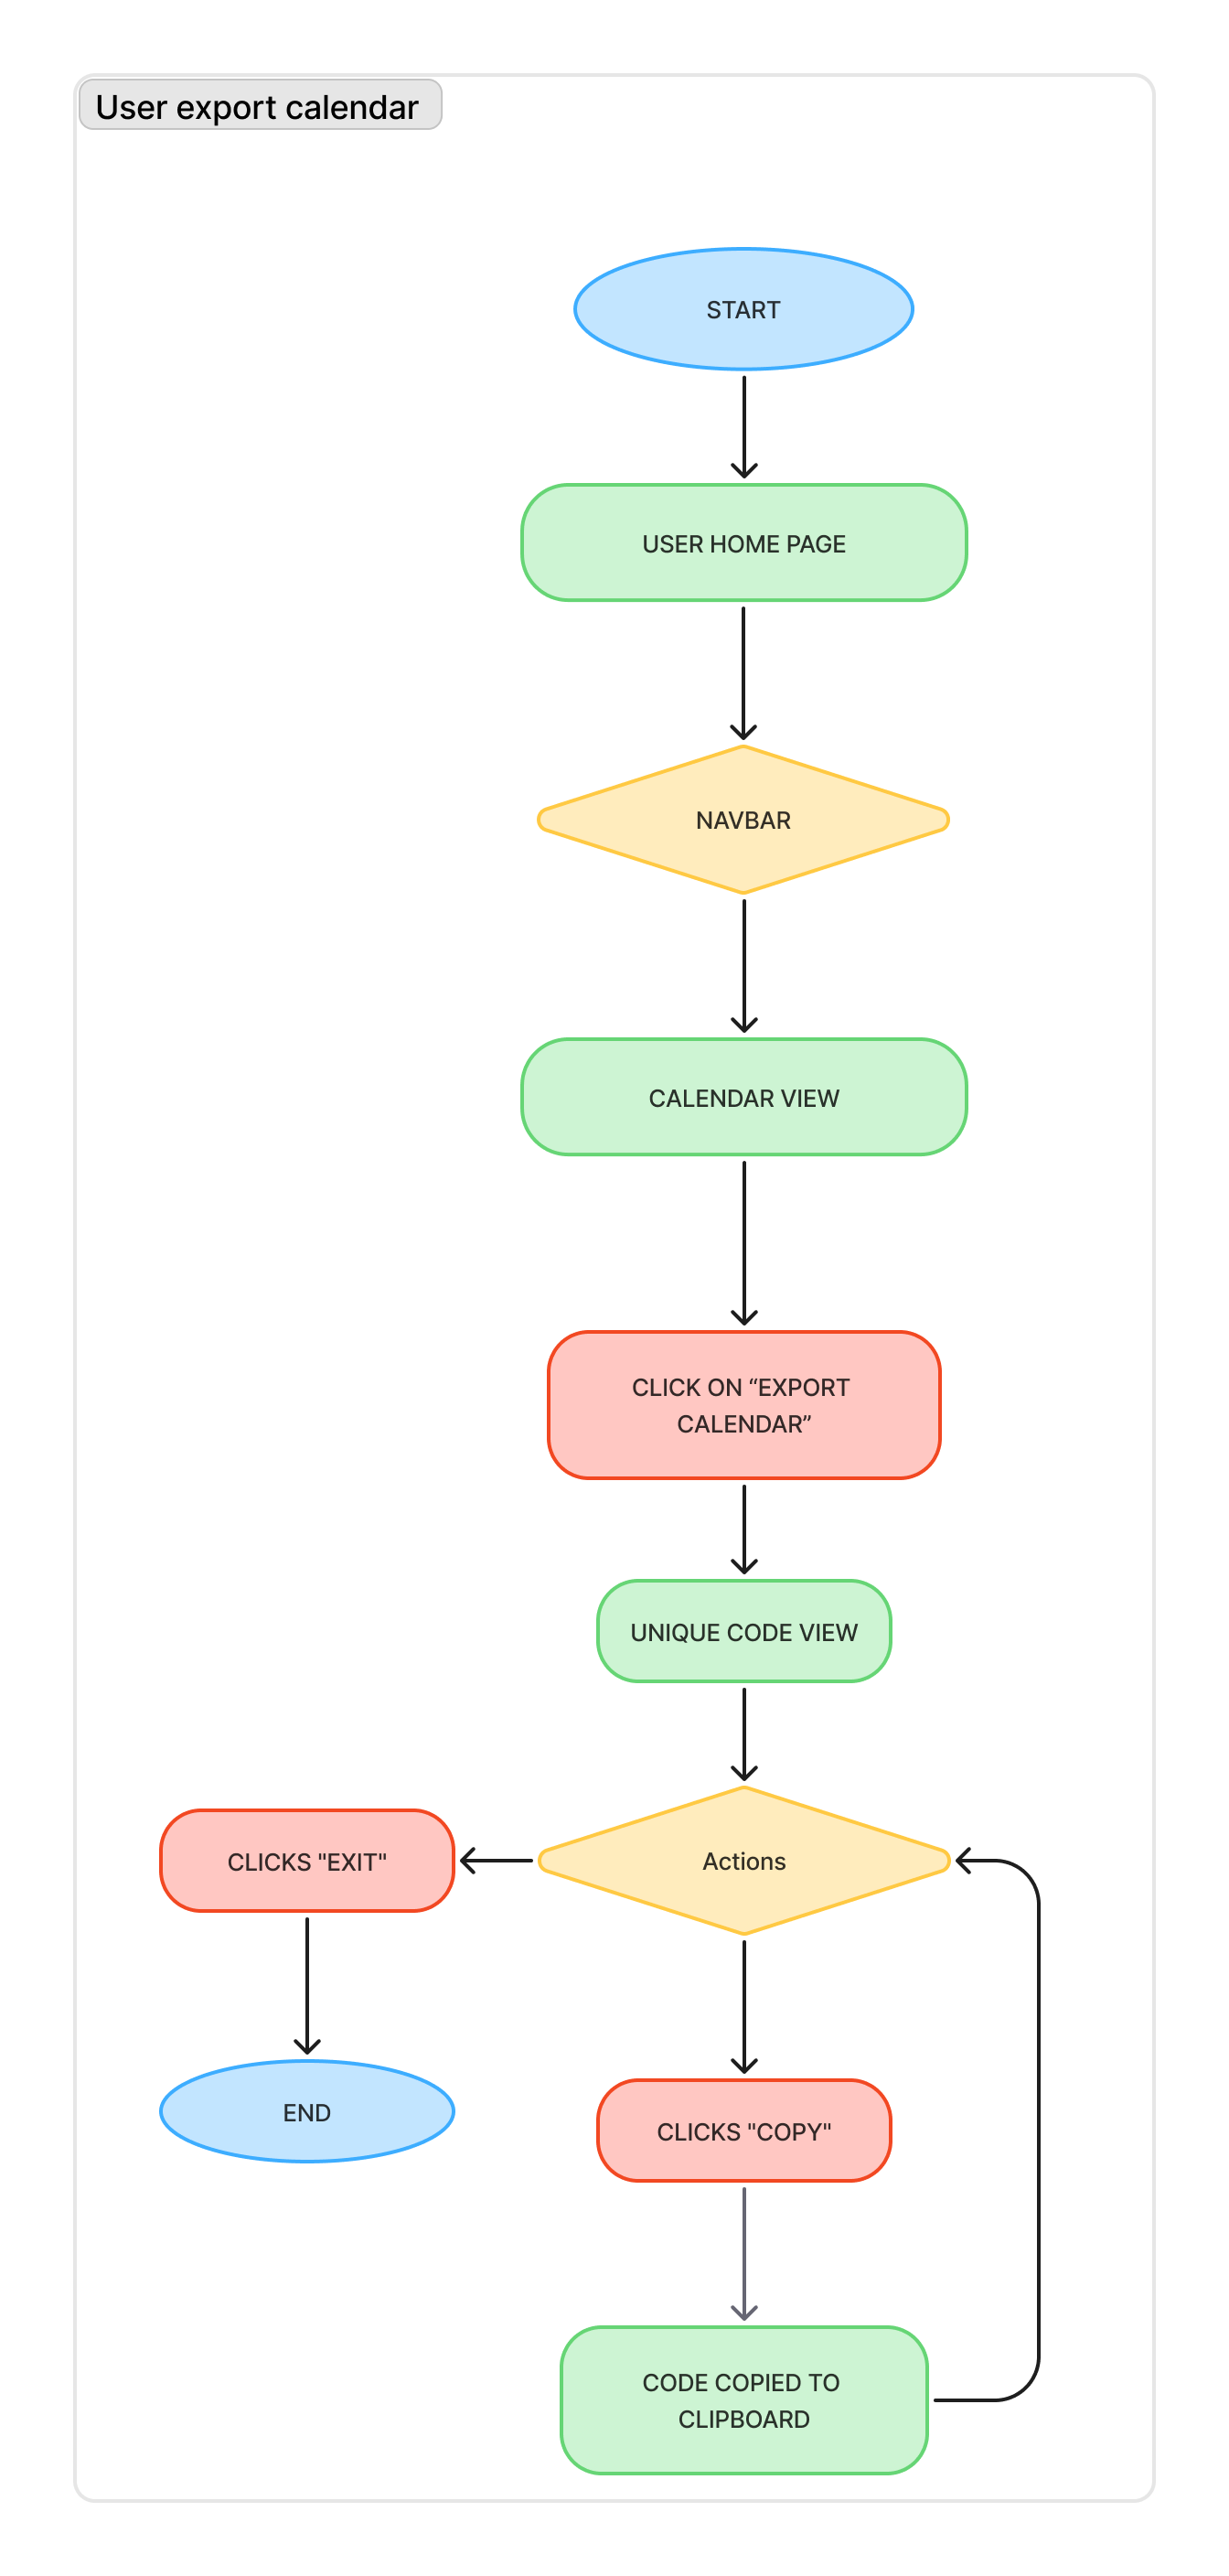
\includegraphics[width=8cm]{User_Flows/ExportCalendar.png}
        \captionof{figure}{User flow regarding Appointment export}
    \end{center}
    %\begin{itemize}   
    %\end{itemize}
\end{minipage}
\vspace{3em}

\begin{minipage}{\textwidth}
    \phantomsection
    \subsection{UF5. Admin - Login}
    The following user flow shows the steps the admin takes to login. UC45 is implemented.
    It refers to use case \textbf{UC45}, and method \textbf{adminLogin(credentials)} from the class \textbf{SystemAdmin} of the class diagram.
    
    \begin{center}
        
\includegraphics[width=8cm]{User_Flows/AdminLogin.png}
        \captionof{figure}{User flow regarding Admin Login}
    \end{center}
    %\begin{itemize}   
    %\end{itemize}
\end{minipage}
\vspace{3em}

\begin{minipage}{\textwidth}
    \phantomsection
    \subsection{UF6. Admin - Create Insurance Policy, Hospital, Treatment, Department. Register Doctor}
    \label{UF6}
    The following user flow shows the steps the admin takes to create an Insurance Policy, Hospital, Treatment, Department and register a Doctor. UC1, UC2, UC12 are implemented.
    It refers to use cases \textbf{UC1, UC2, UC12}, and methods \textbf{InsurancePolicy.create(policyData), Hospital.create(hospitalData), Treatment.create(treatmentData), SystemAdmin.createDepartment(hospital, departmentData), SystemAdmin.registerDoctor(doctorData)} from the classes \textbf{InsurancePolicy, Hospital, Treatment, SystemAdmin} of the class diagram.
    
    \begin{center}
        
\includegraphics[width=0.8\textwidth]{User_Flows/CreatePolicyHospitalTreatmentDepartment.png}
        \captionof{figure}{User flow regarding Admin Create Insurance Policy, Hospital, Treatment, Department. Register Doctor}
    \end{center}
    %\begin{itemize}   
    %\end{itemize}
\end{minipage}
\vspace{3em}

\begin{minipage}{\textwidth}
    \phantomsection
    \subsection{UF7. Admin - Edit Insurance Policy, Hospital, Treatment, Department}
    \label{UF7}
    The following user flow shows the steps the admin takes to edit an Insurance Policy, Hospital, Treatment, Department. UC5 and UC6 are implemented.
    It refers to use cases \textbf{UC5, UC6}, and methods \textbf{InsurancePolicy.edit(policy, newPolicyData), Hospital.edit(hospital, newHospitalData), Treatment.edit(treatment, newTreatmentData), Department.edit(department, newDepartmentData)} from the classes \textbf{InsurancePolicy, Hospital, Treatment, Department} of the class diagram.
    
    \begin{center}
        
\includegraphics[width=0.8\textwidth]{User_Flows/EditPolicyHospitalTreatmentDepartment.png}
        \captionof{figure}{User flow regarding Edit Insurance Policy, Hospital, Treatment, Department}
    \end{center}
    %\begin{itemize}   
    %\end{itemize}
\end{minipage}
\vspace{3em}

\begin{minipage}{\textwidth}
    \phantomsection
    \subsection{UF8. Admin - Deactivate Insurance Policy, Hospital, Treatment, Department}
    \label{UF8}
    The following user flow shows the steps the admin takes to deactivate an Insurance Policy, Hospital, Treatment, Department. UC8 and UC9 are implemented.
    It refers to use cases \textbf{UC8, UC9}, and methods \textbf{InsurancePolicy.deactivate(policy), Hospital.close(), Treatment.deactivate(), Department.close()} from the classes \textbf{InsurancePolicy, Hospital, Treatment, Department} of the class diagram.
    
    \begin{center}
        
\includegraphics[width=0.8\textwidth]{User_Flows/DeactivatePolicyHospitalTreatmentDepartment.png}
        \captionof{figure}{User flow regarding Deactivate Insurance Policy, Hospital, Treatment, Department}
    \end{center}
    %\begin{itemize}   
    %\end{itemize}
\end{minipage}
\vspace{3em}

\begin{minipage}{\textwidth}
    \phantomsection
    \subsection{UF9. Admin - Appoint Head of Hospital}
    The following user flow shows the steps the admin takes to appoint a Head of Hospital. UC14 is implemented.
    It refers to use case \textbf{UC14}, and methods \textbf{appointHeadOfHospital(doctor, hospital)} from the class \textbf{SystemAdmin} of the class diagram.
    
    \begin{center}
        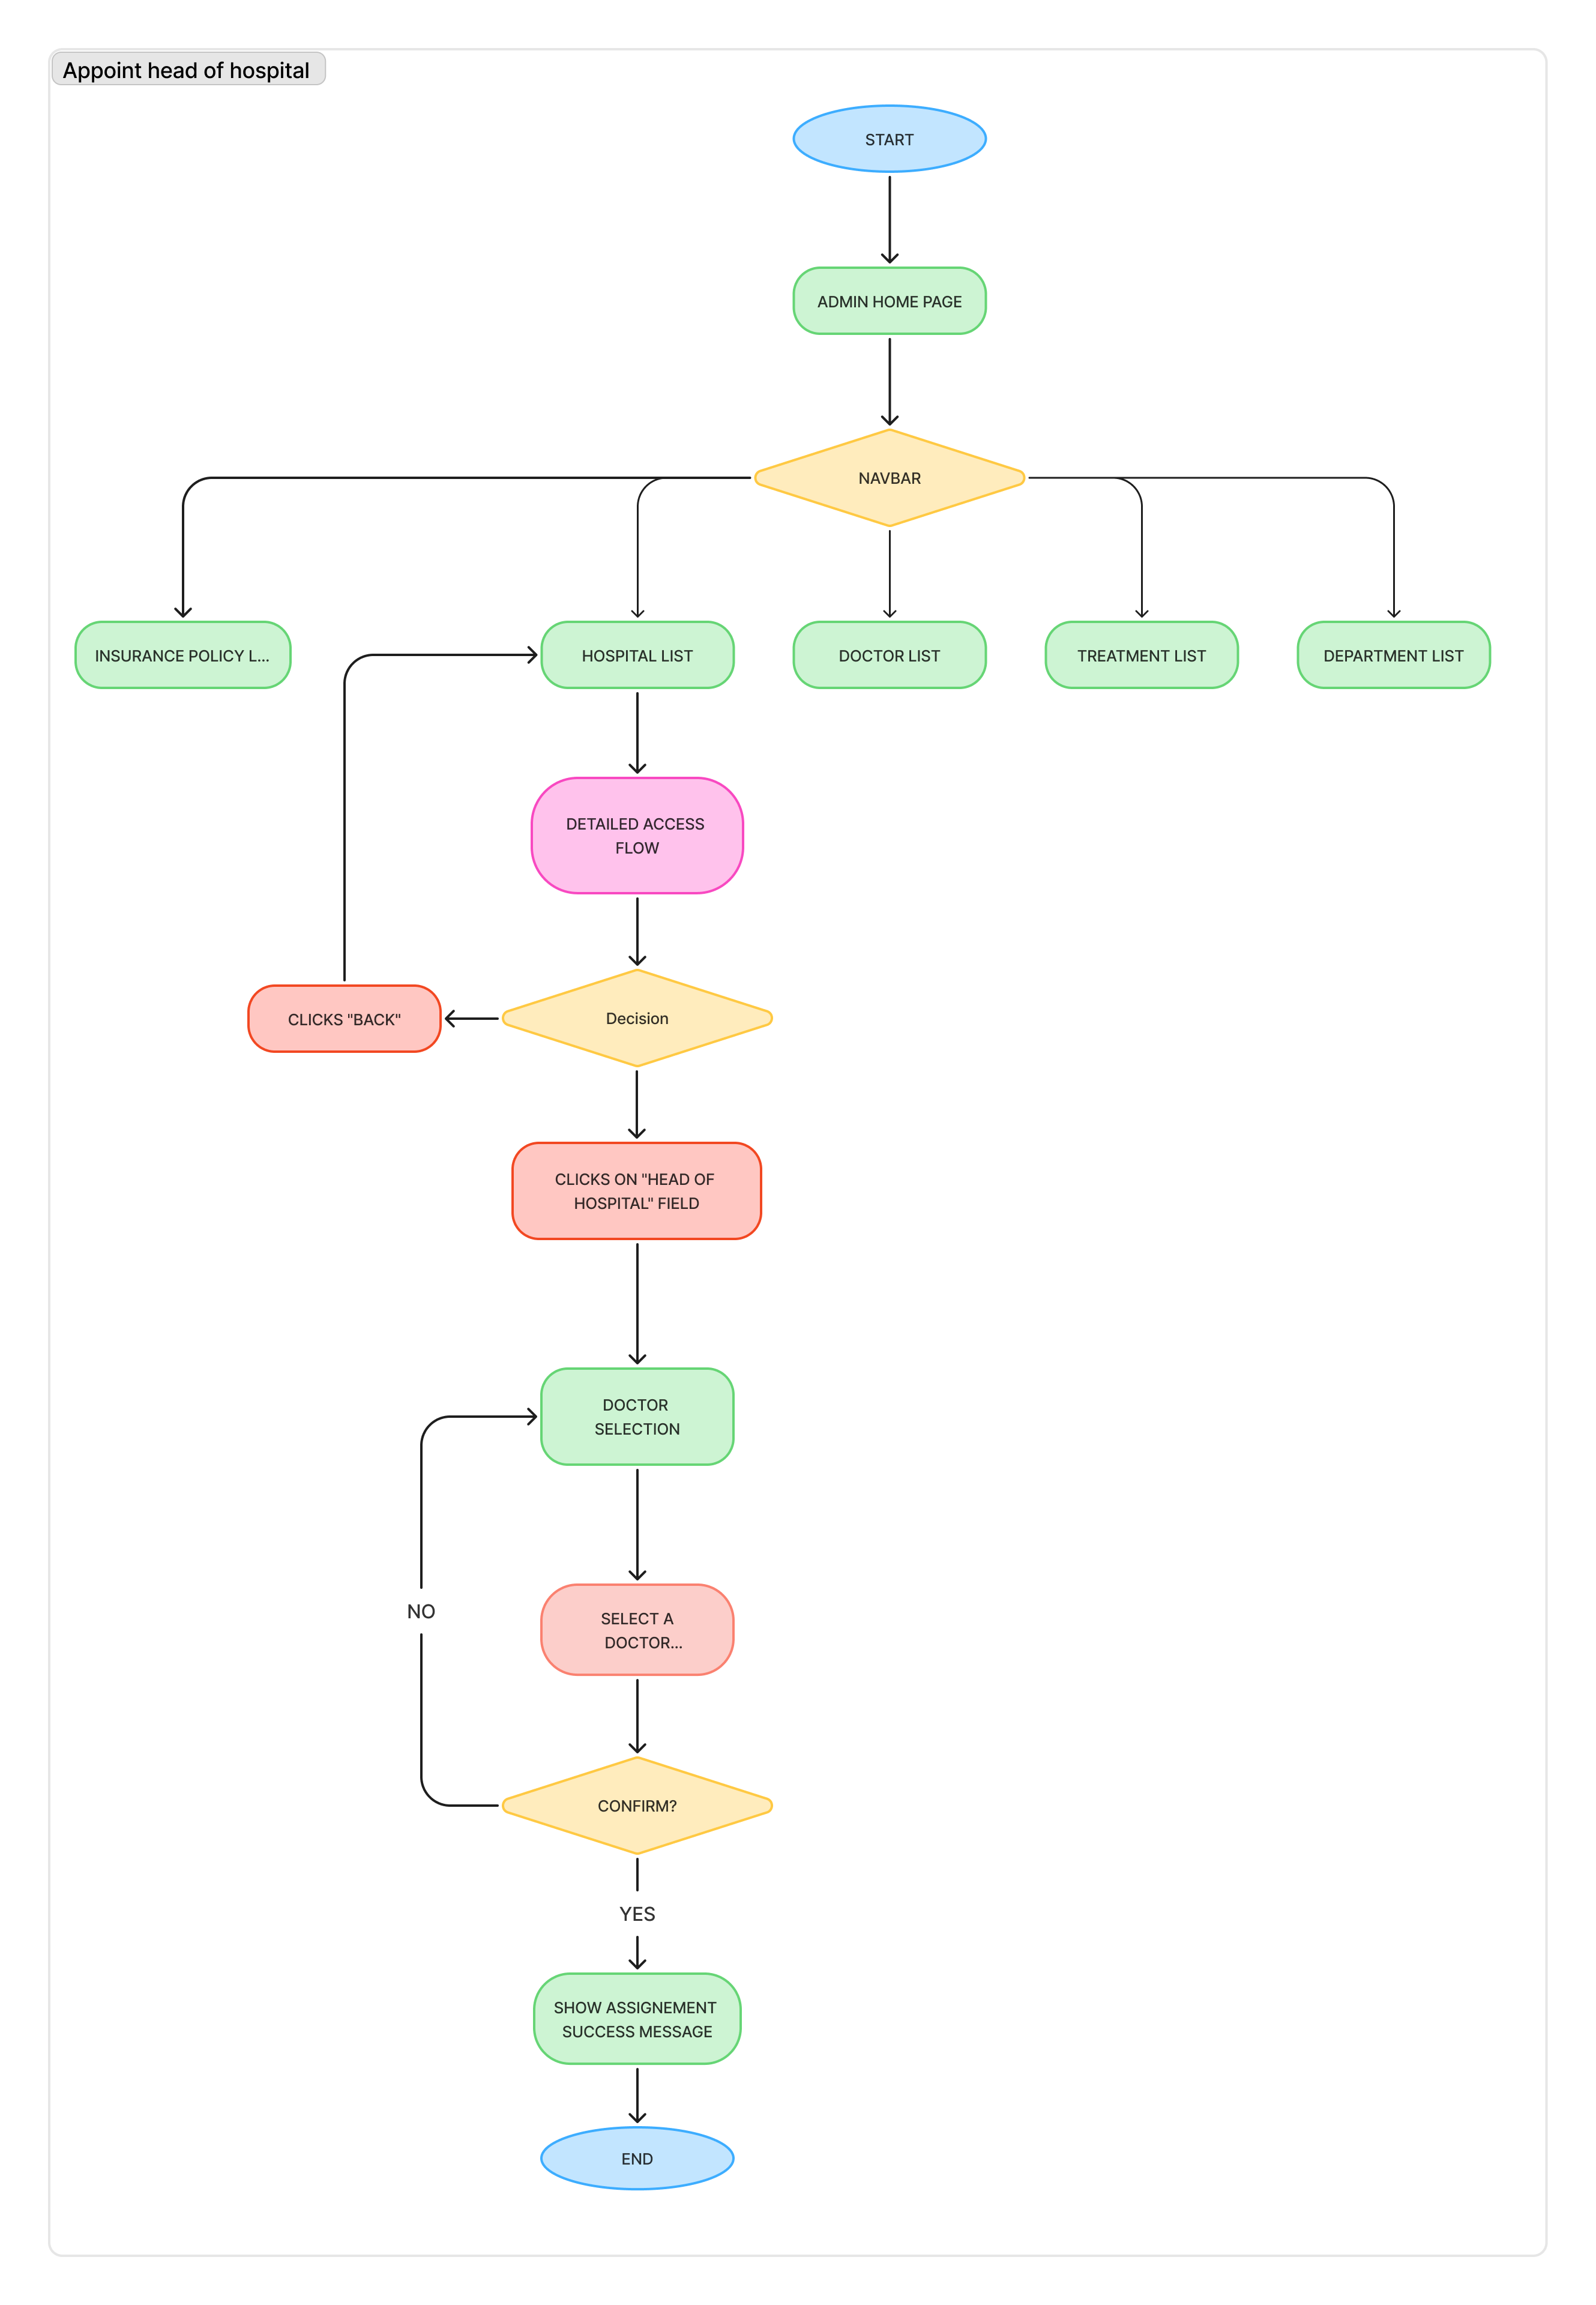
\includegraphics[width=0.8\textwidth]{User_Flows/AppointHeadOfHospital.png}
        \captionof{figure}{User flow regarding Appoint Head of Hospital}
    \end{center}
    %\begin{itemize}   
    %\end{itemize}
\end{minipage}
\vspace{3em}

\begin{minipage}{\textwidth}
    \phantomsection
    \subsection{UF10. Admin - Assign Doctor to Hospital}
    The following user flow shows the steps the admin takes to assign a doctor to a hospital. UC13 is implemented. 
    It refers to use case \textbf{UC13}, and methods \textbf{assignDoctorToHospital(doctor, hospital)} from the class \textbf{SystemAdmin} of the class diagram.
    
    \begin{center}
        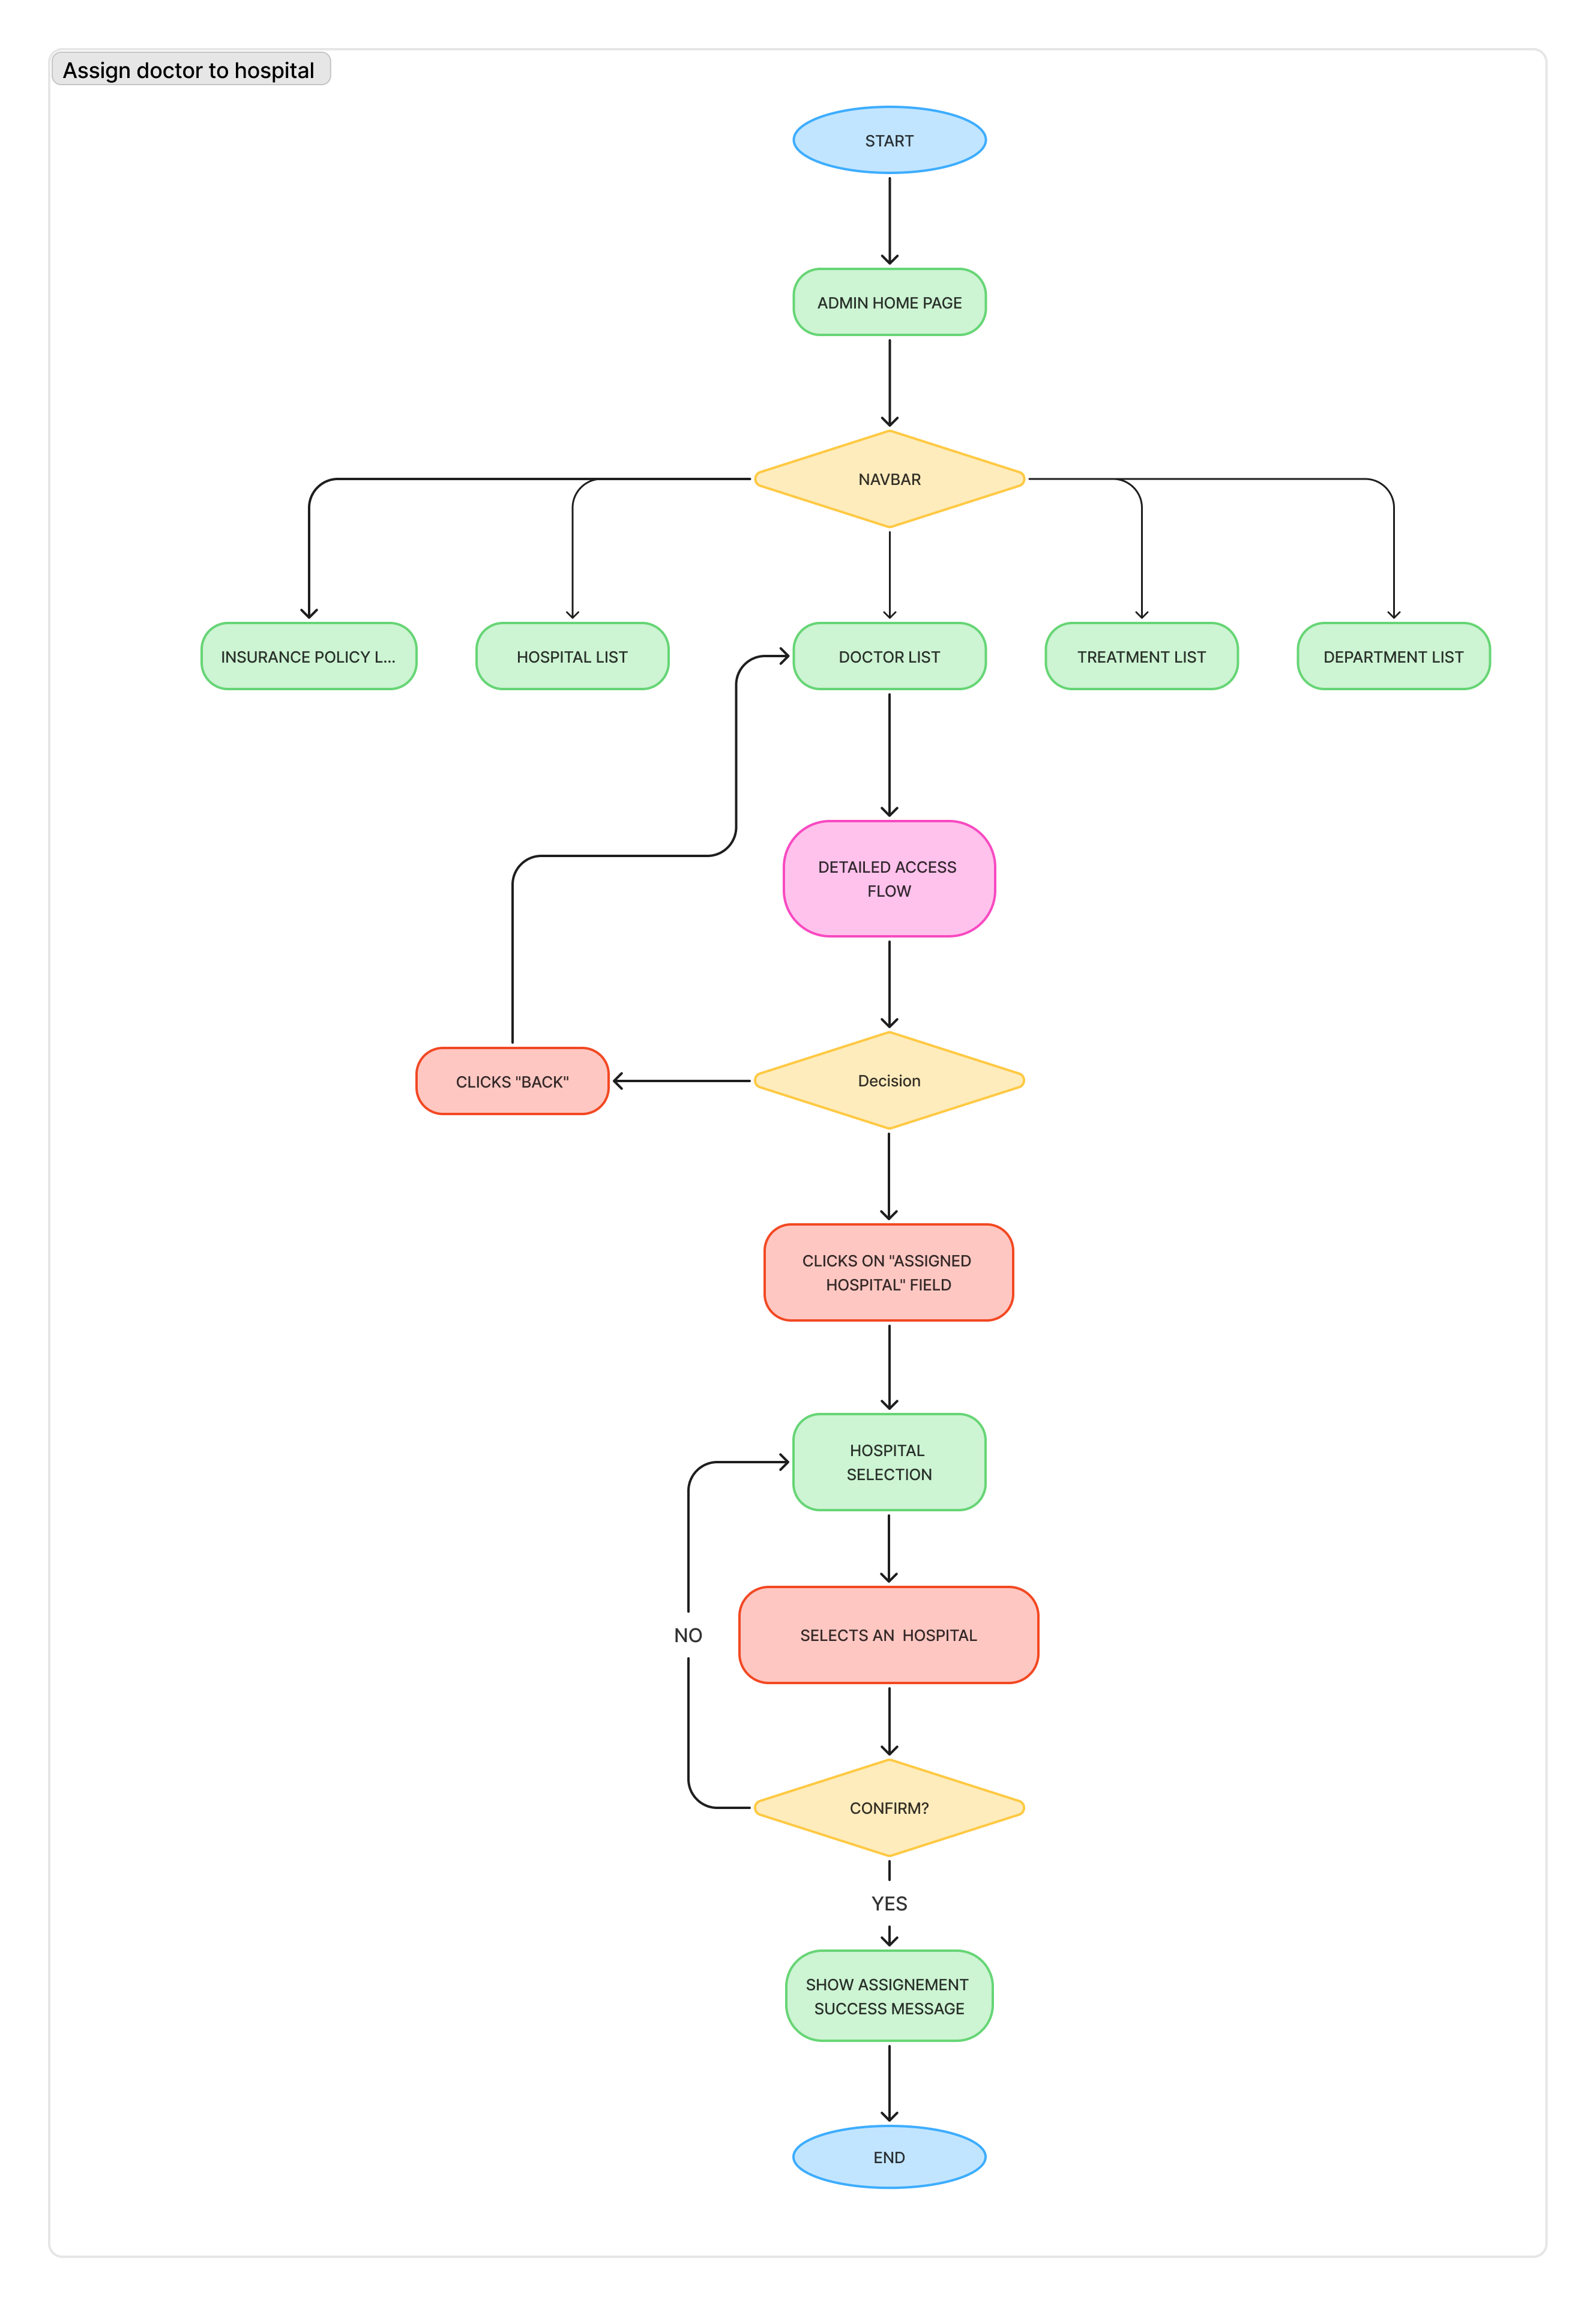
\includegraphics[width=0.8\textwidth]{User_Flows/AssignDoctorHospital.png}
        \captionof{figure}{User flow regarding Assign Doctor to Hospital}
    \end{center}
    %\begin{itemize}   
    %\end{itemize}
\end{minipage}
\vspace{3em}

\begin{minipage}{\textwidth}
    \phantomsection
    \subsection{UF11. Admin - Generate Unique Code}
    The following user flow shows the steps the admin takes to generate a unique insurance policy code. UC22 is implemented.
    It refers to use case \textbf{UC22}, and methods \textbf{generateCode()} from the class \textbf{InsurancePolicy} of the class diagram.
    
    \begin{center}
        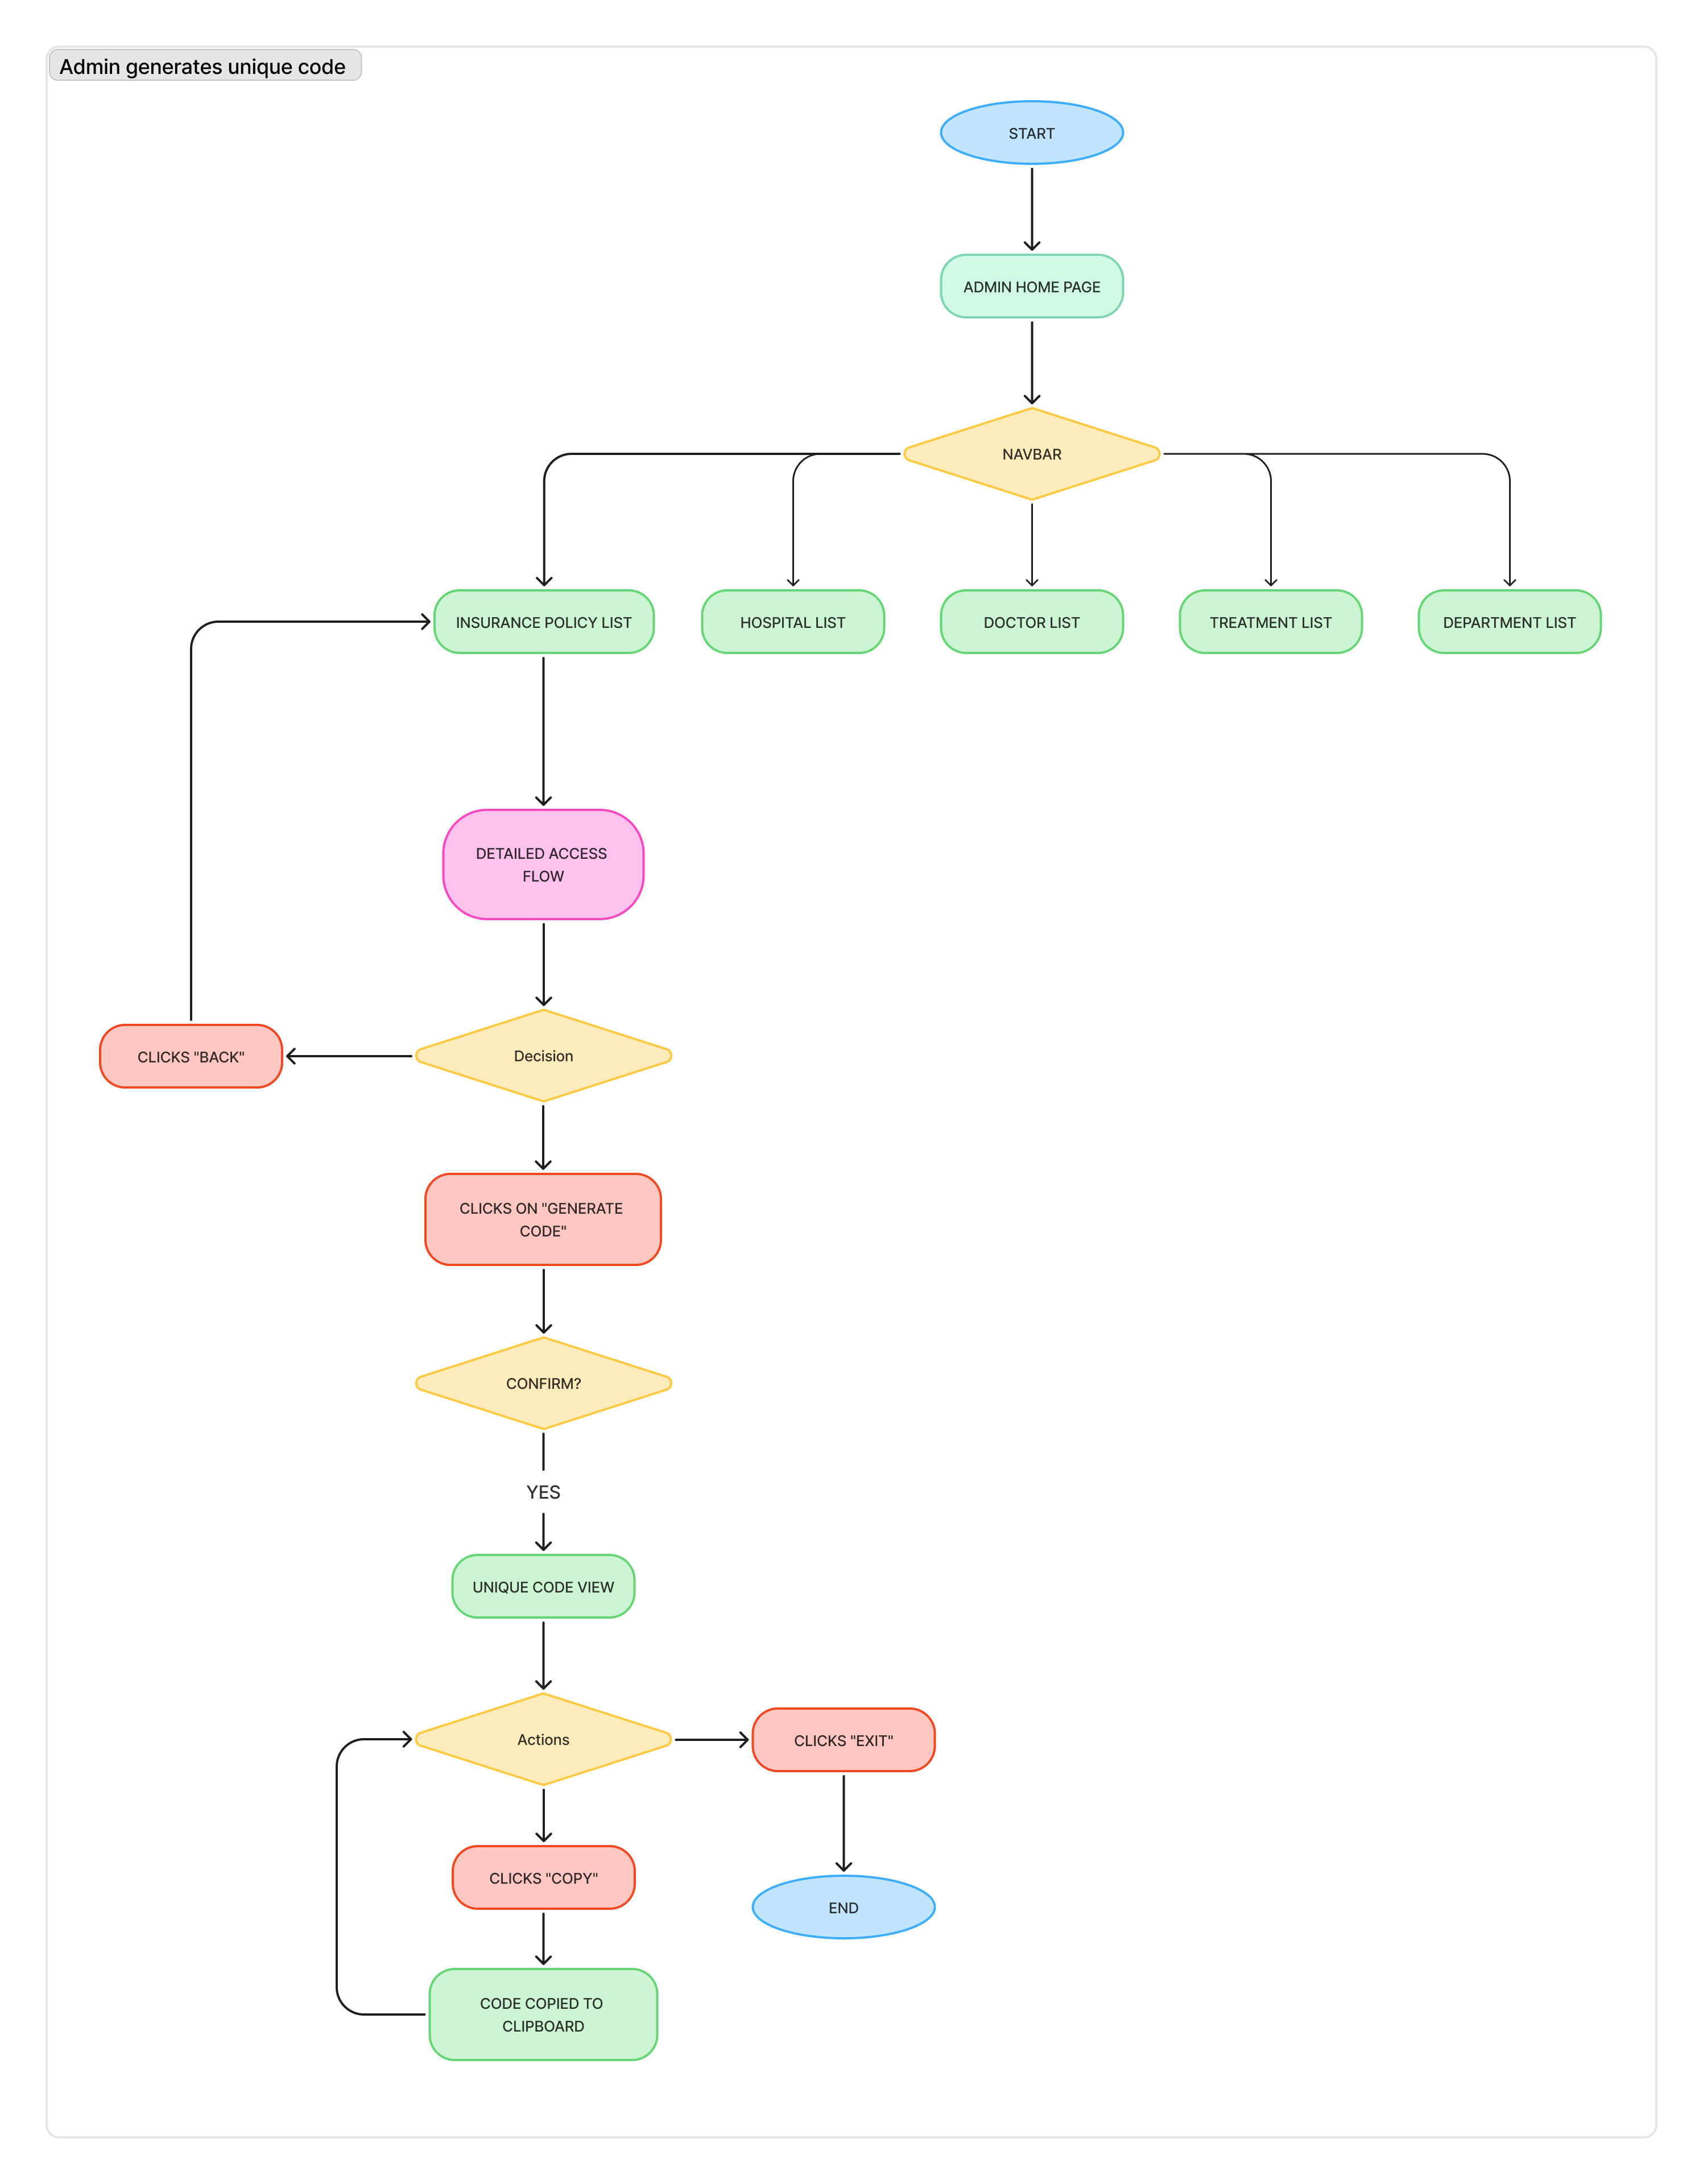
\includegraphics[width=0.8\textwidth]{User_Flows/GenerateUniqueCode.png}
        \captionof{figure}{User flow regarding Generate Unique Code}
    \end{center}
    %\begin{itemize}   
    %\end{itemize}
\end{minipage}
\vspace{3em}

\begin{minipage}{\textwidth}
    \phantomsection
    \subsection{UF12. Patient - Registration and Validation}
    \label{UF12}
    The following user flow shows the process of Patient registration and validation. UC23 is implemented.
    It refers to use case \textbf{UC23}, and methods \textbf{register(userData), validateAccount(token)} from the class \textbf{Patient} of the class diagram.
    
    \begin{center}
        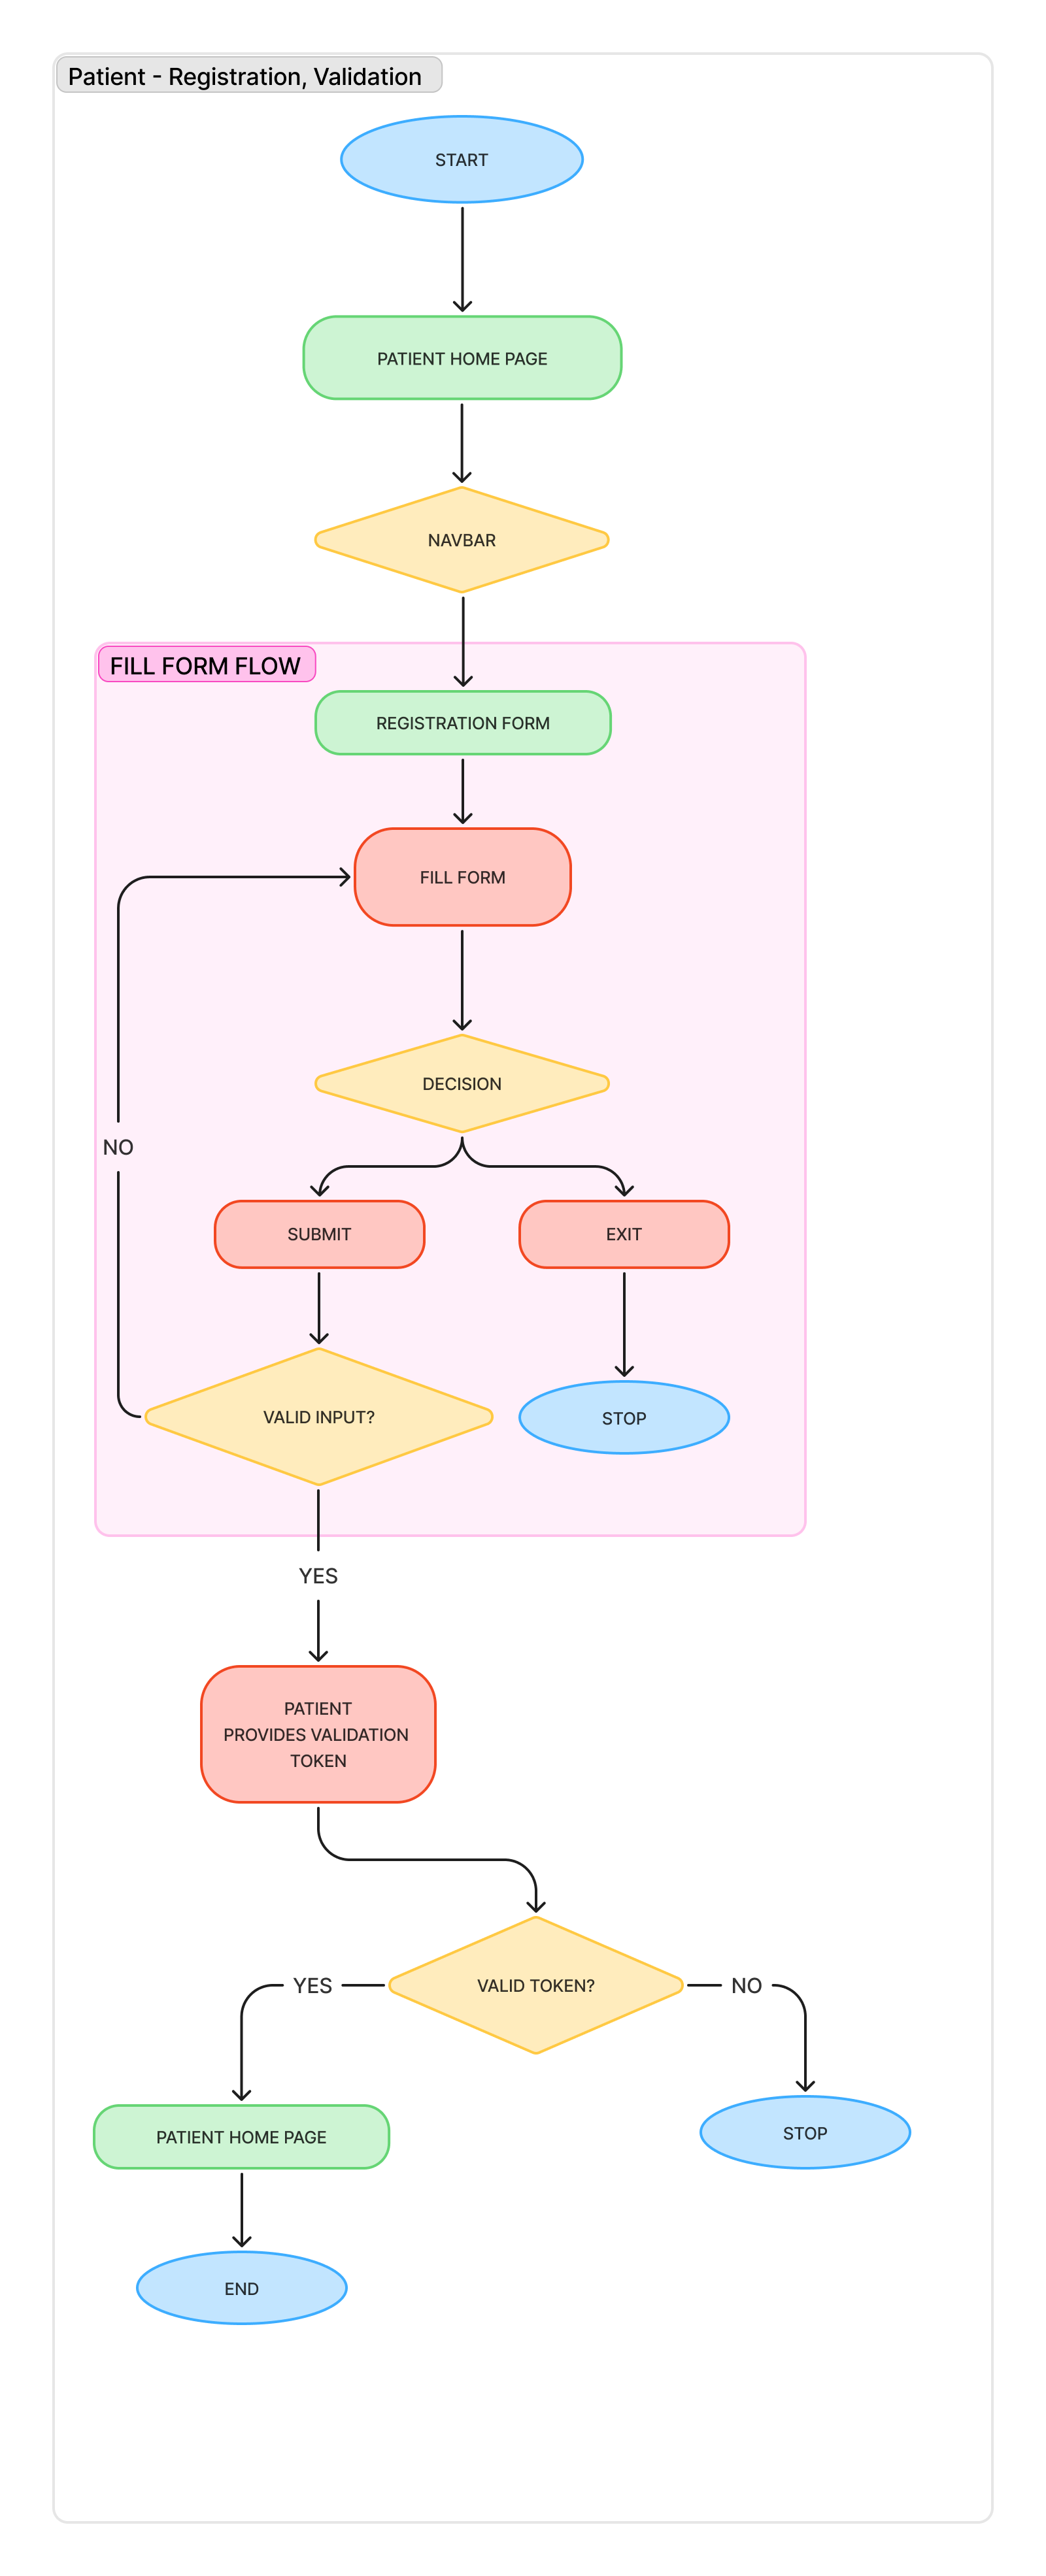
\includegraphics[width=8cm]{User_Flows/PatientRegistrationValidation.png}
        \captionof{figure}{User flow regarding Patient Registration and Validation}
    \end{center}
    %\begin{itemize}   
    %\end{itemize}
\end{minipage}
\vspace{3em}

\begin{minipage}{\textwidth}
    \phantomsection
    \subsection{UF13. Patient - Appointment Cancellation and Rescheduling}
    The following user flow shows the steps a patient takes to cancel and reschedule an appointment. UC10 is implemented, while UC29 is not.
    It refers to use cases \textbf{UC10, UC29}, and methods \textbf{cancel(), reschedule(newDateTime)} from the class \textbf{Appointment} of the class diagram.
    
    \begin{center}
        
\includegraphics[width=0.8\textwidth]{User_Flows/PatientCancellationRescheduling.png}
        \captionof{figure}{User flow regarding Patient Appointment Cancellation and Rescheduling}
    \end{center}
    %\begin{itemize}   
    %\end{itemize}
\end{minipage}
\vspace{3em}

\begin{minipage}{\textwidth}
    \phantomsection
    \subsection{UF14. Patient - Appointment Booking and Payment}
    The following user flow shows the steps a patient takes to book and pay an appointment. UC27 is implemented while UC32 and UC35 are not.
    It refers to use cases \textbf{UC27, UC32, UC35}, and methods \textbf{Appointment.book(treatment,hospital,datetime), Payment.pay(paymentData)} from the classes \textbf{Appointment, Payment} of the class diagram.
    
    \begin{center}
        
\includegraphics[width=0.8\textwidth]{User_Flows/AppointmentBookingPayment.png}
        \captionof{figure}{User flow regarding Patient Appointment Booking and Payment}
    \end{center}
    %\begin{itemize}   
    %\end{itemize}
\end{minipage}
\vspace{3em}

\begin{minipage}{\textwidth}
    \phantomsection
    \subsection{UF15. Patient - Register Insurance Policy via unique code}
    The following user flow shows the steps a patient takes to add an insurance policy to their profile via unique code. UC36 is not implemented.
    It refers to use case \textbf{UC36}, and methods \textbf{registerInsurance(code)} from the class \textbf{Patient} of the class diagram.
    
    \begin{center}
        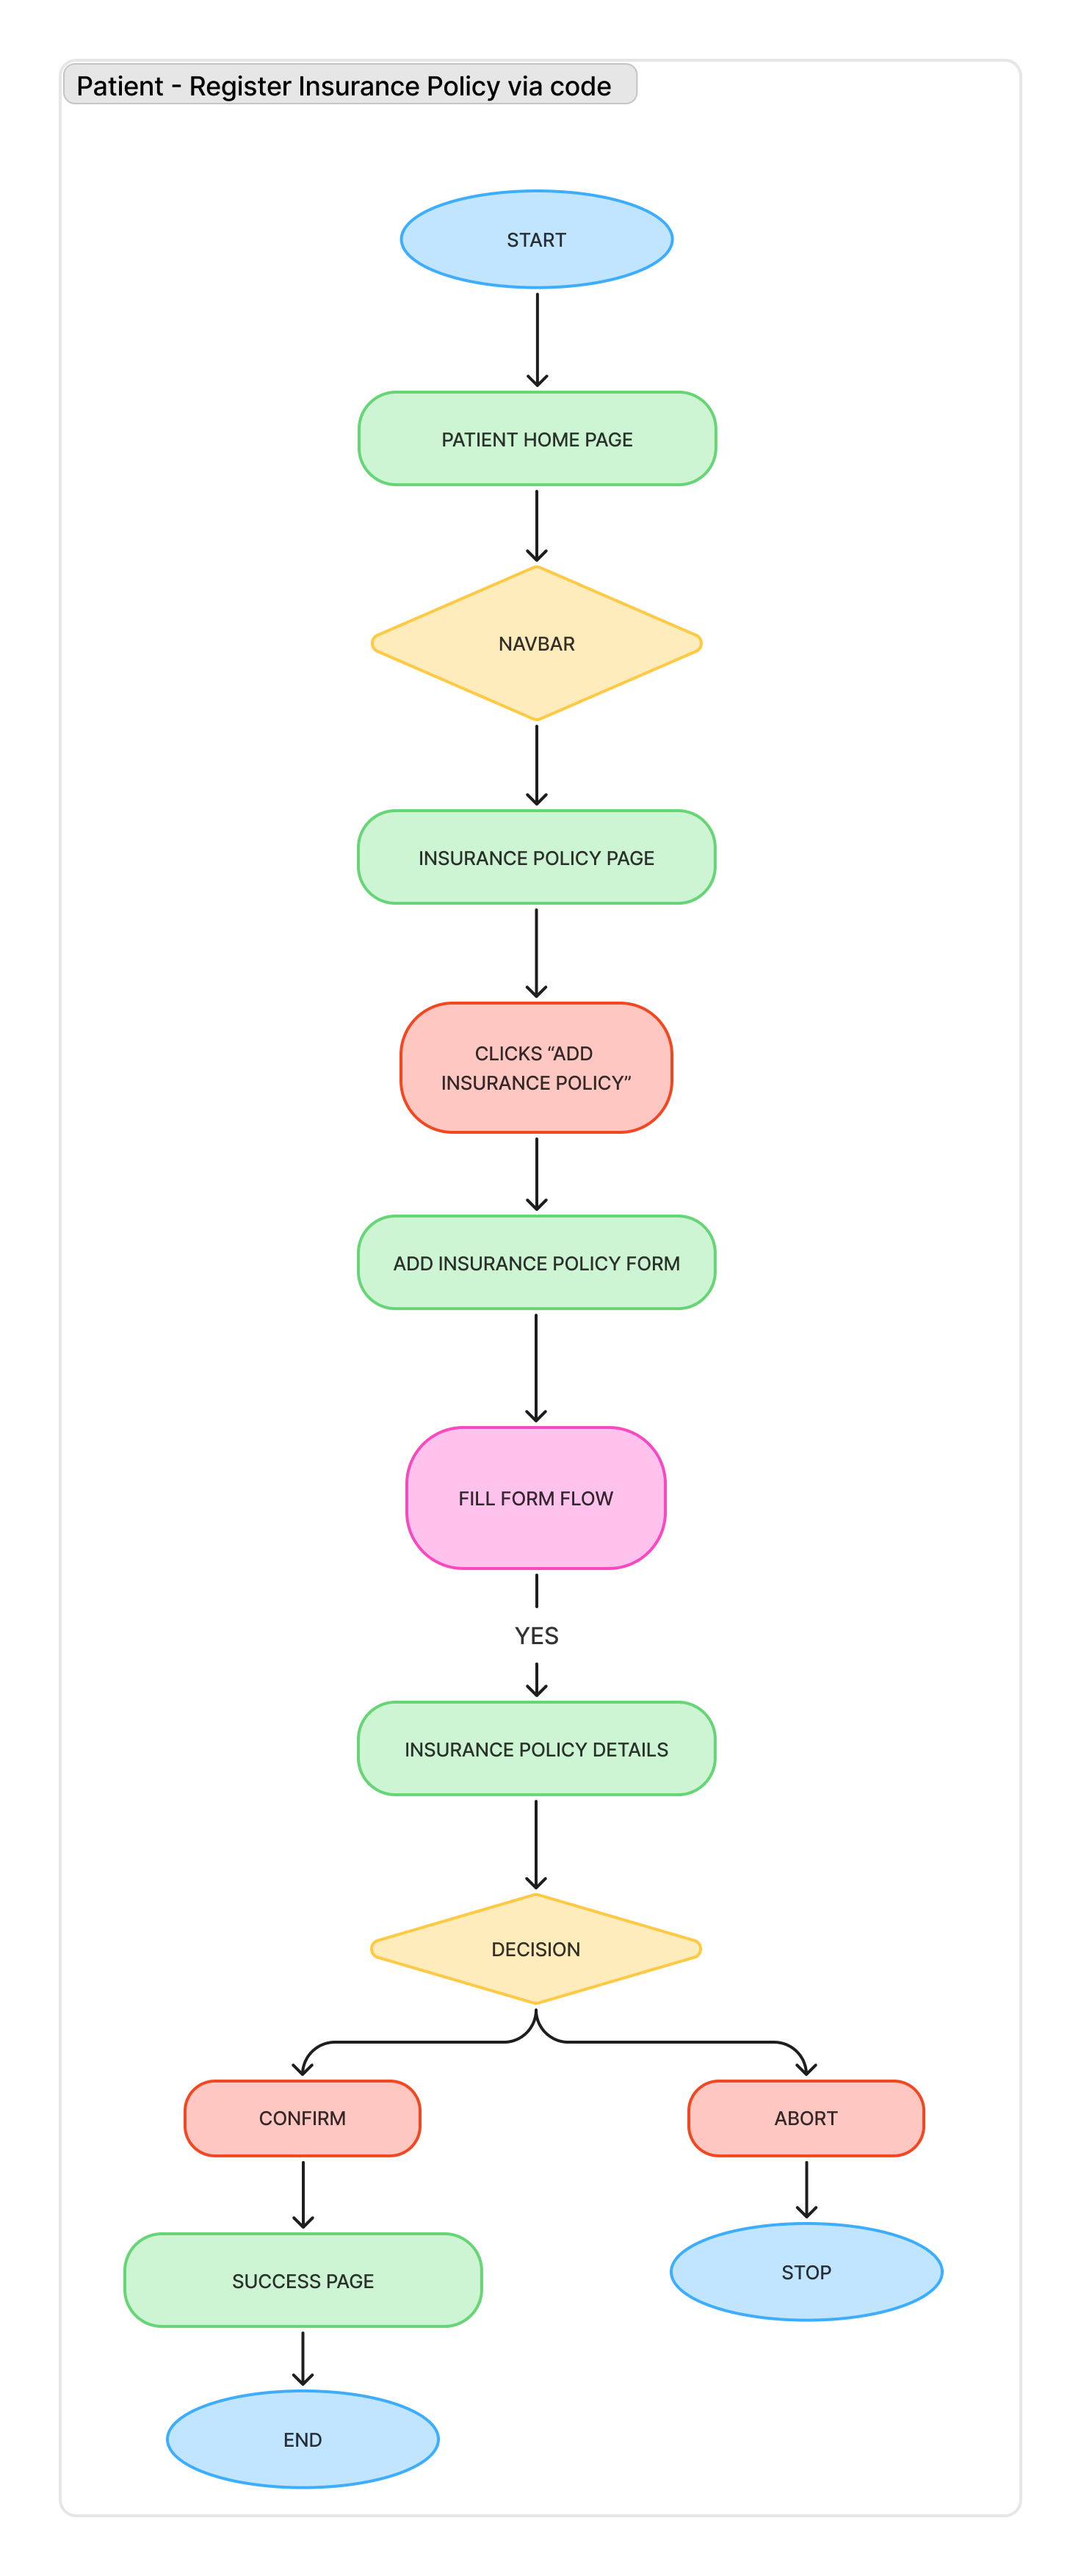
\includegraphics[width=0.5\textwidth]{User_Flows/PatientRegisterPolicy.png}
        \captionof{figure}{User flow regarding Patient Register Insurance Policy via unique code}
    \end{center}
    %\begin{itemize}   
    %\end{itemize}
\end{minipage}
\vspace{3em}

\begin{minipage}{\textwidth}
    \phantomsection
    \subsection{UF16. Patient - Medical Record and Prescriptions consultation}
    \label{UF16}
    The following user flow shows the steps a patient takes to view their medical record and prescriptions in detail. UC38, UC39 and UC40 are implemented.
    It refers to use cases \textbf{UC38, UC39, UC40}, and methods \textbf{Patient.getPrescriptions(), Prescription.getDetails(), Patient.getMedicalRecord()} from the classes \textbf{Patient, Prescription} of the class diagram.
    
    \begin{center}
        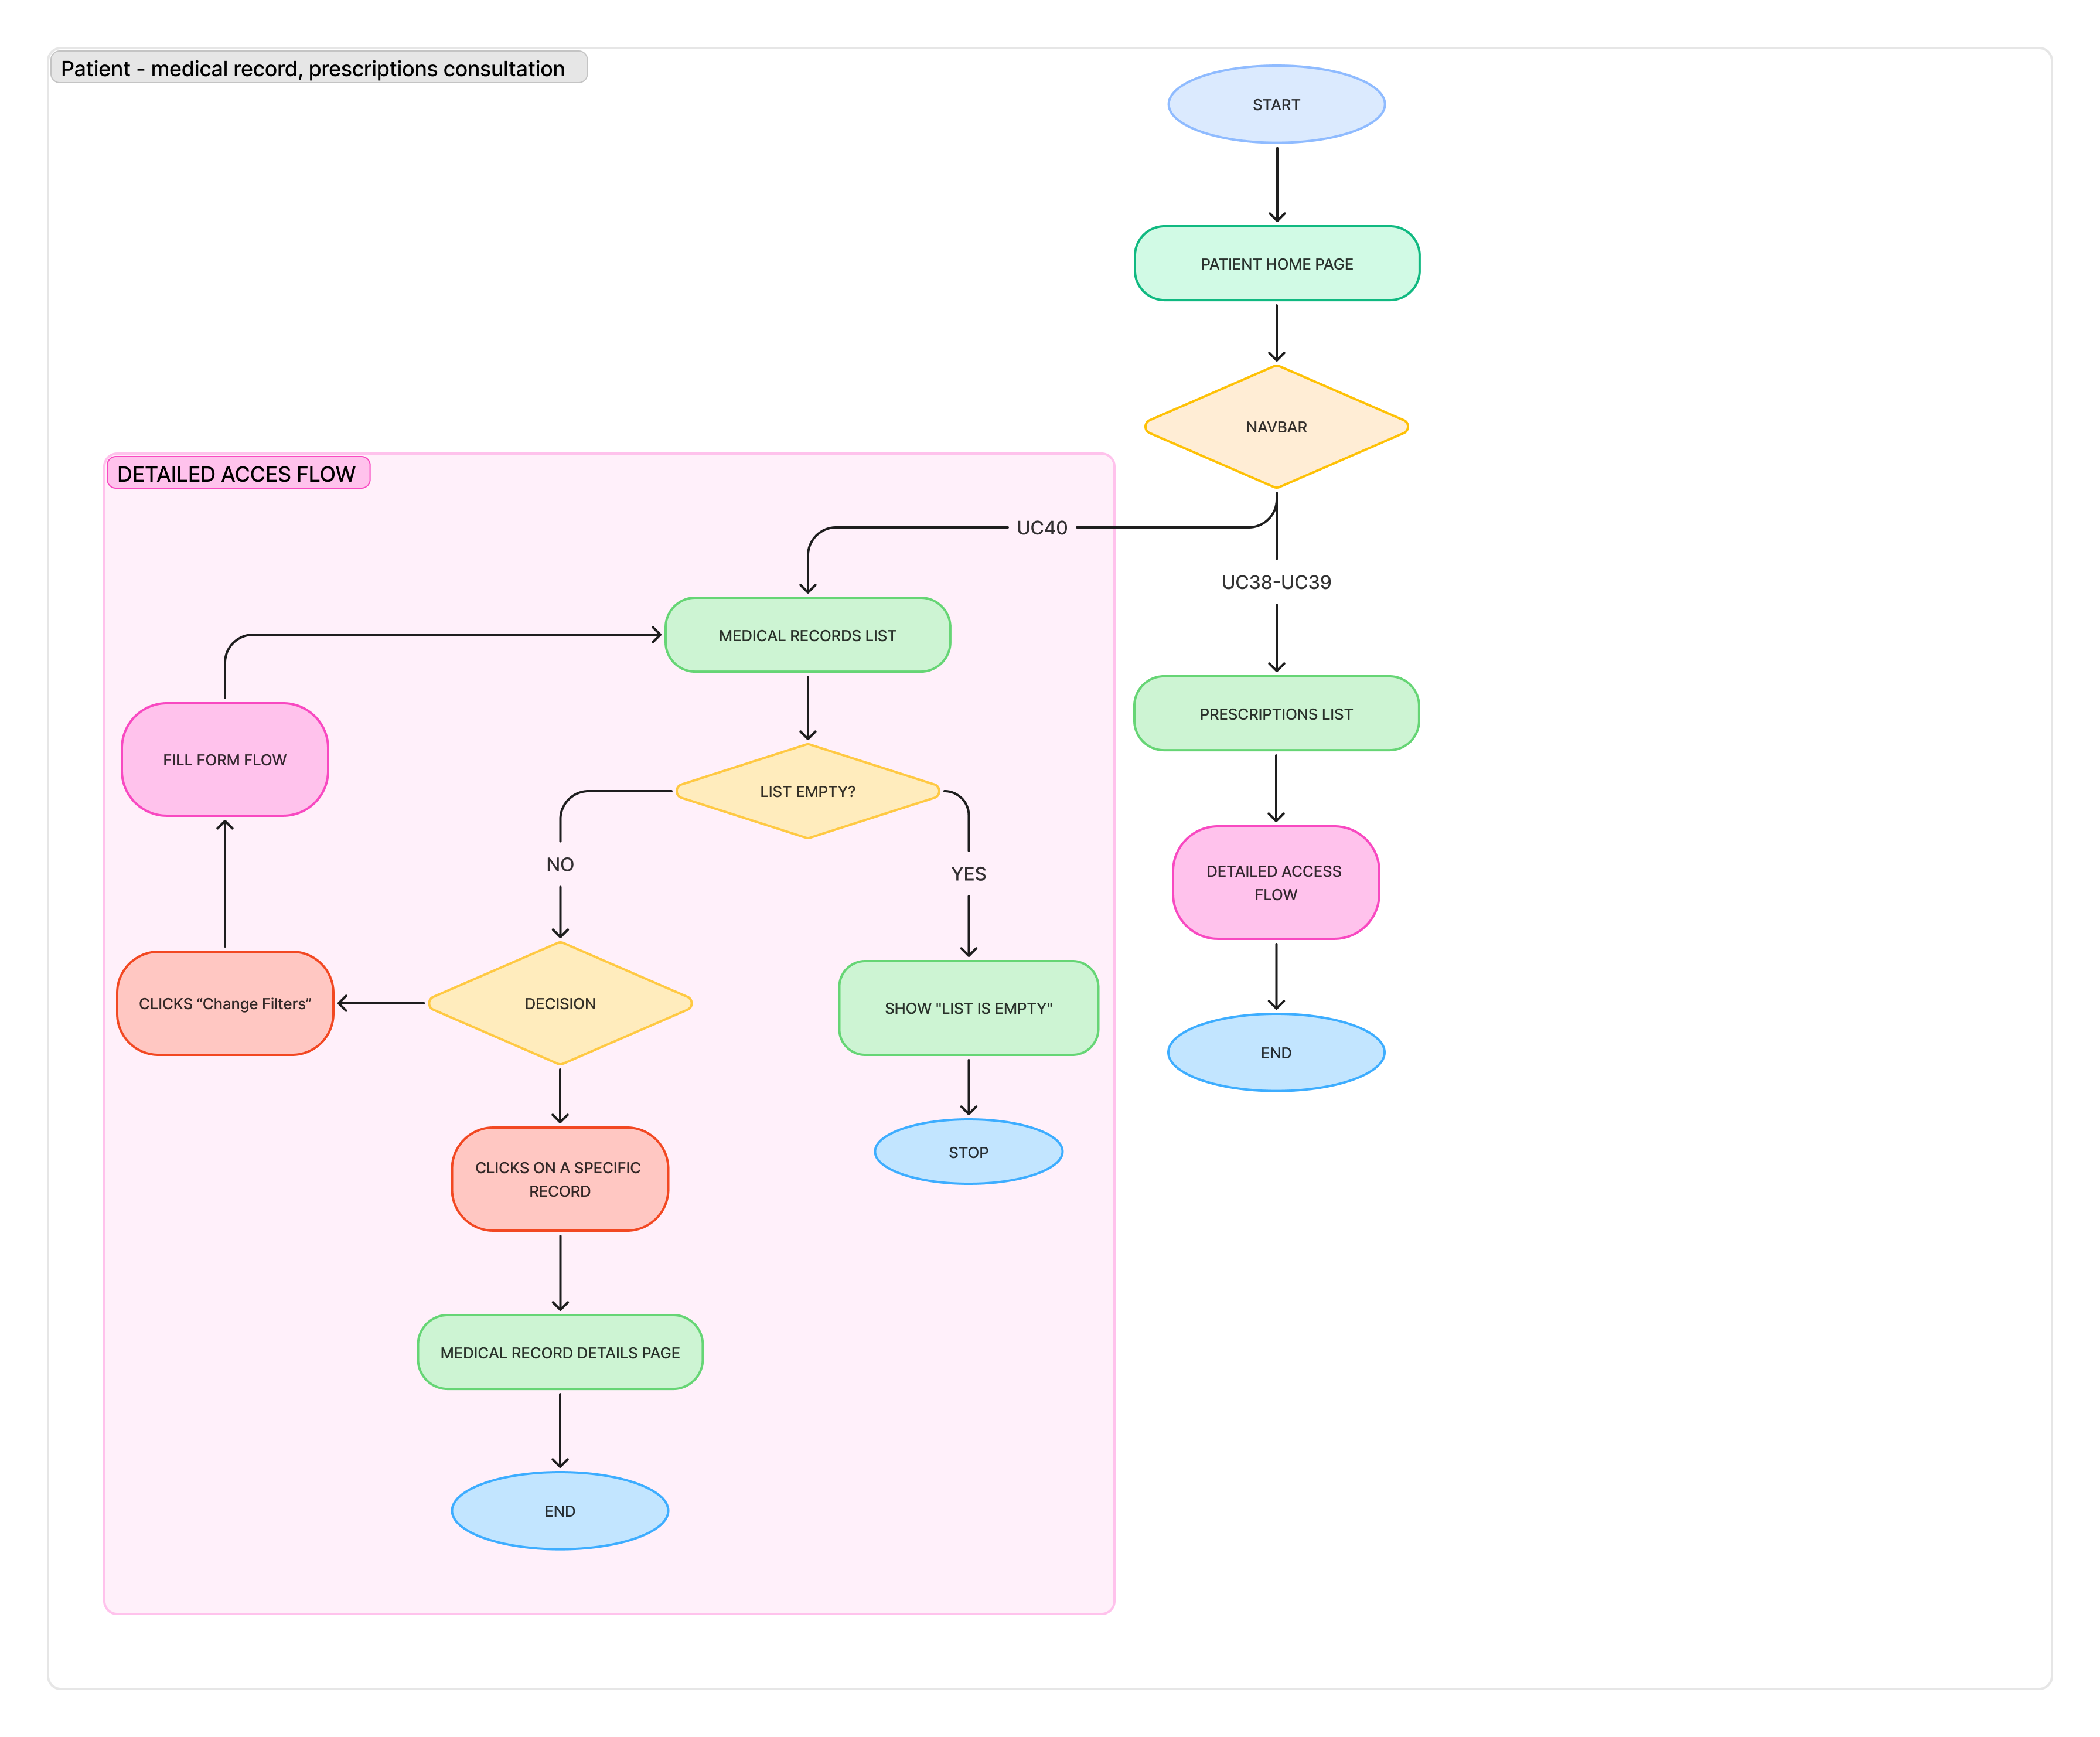
\includegraphics[width=0.9\textwidth]{User_Flows/PatientMedicalRecordPrescriptionExemptions.png}
        \captionof{figure}{User flow regarding Patient Medical Record and Prescriptions consultation}
    \end{center}
    %\begin{itemize}   
    %\end{itemize}
\end{minipage}
\vspace{3em}

\begin{minipage}{\textwidth}    
    \phantomsection
    \subsection{UF17. Doctor - Access Patient's Medical Record, Chronological Report}
    The following user flow shows the steps a doctor takes to access a patient's medical records and to consult their own chronological report. UC42 and UC43 are implemented.
    It refers to use cases \textbf{UC42, UC43}, and methods \textbf{accessPatientRecord(fiscalCode),viewChronologicalReport()} from the class \textbf{Doctor} of the class diagram.
    
    \begin{center}
        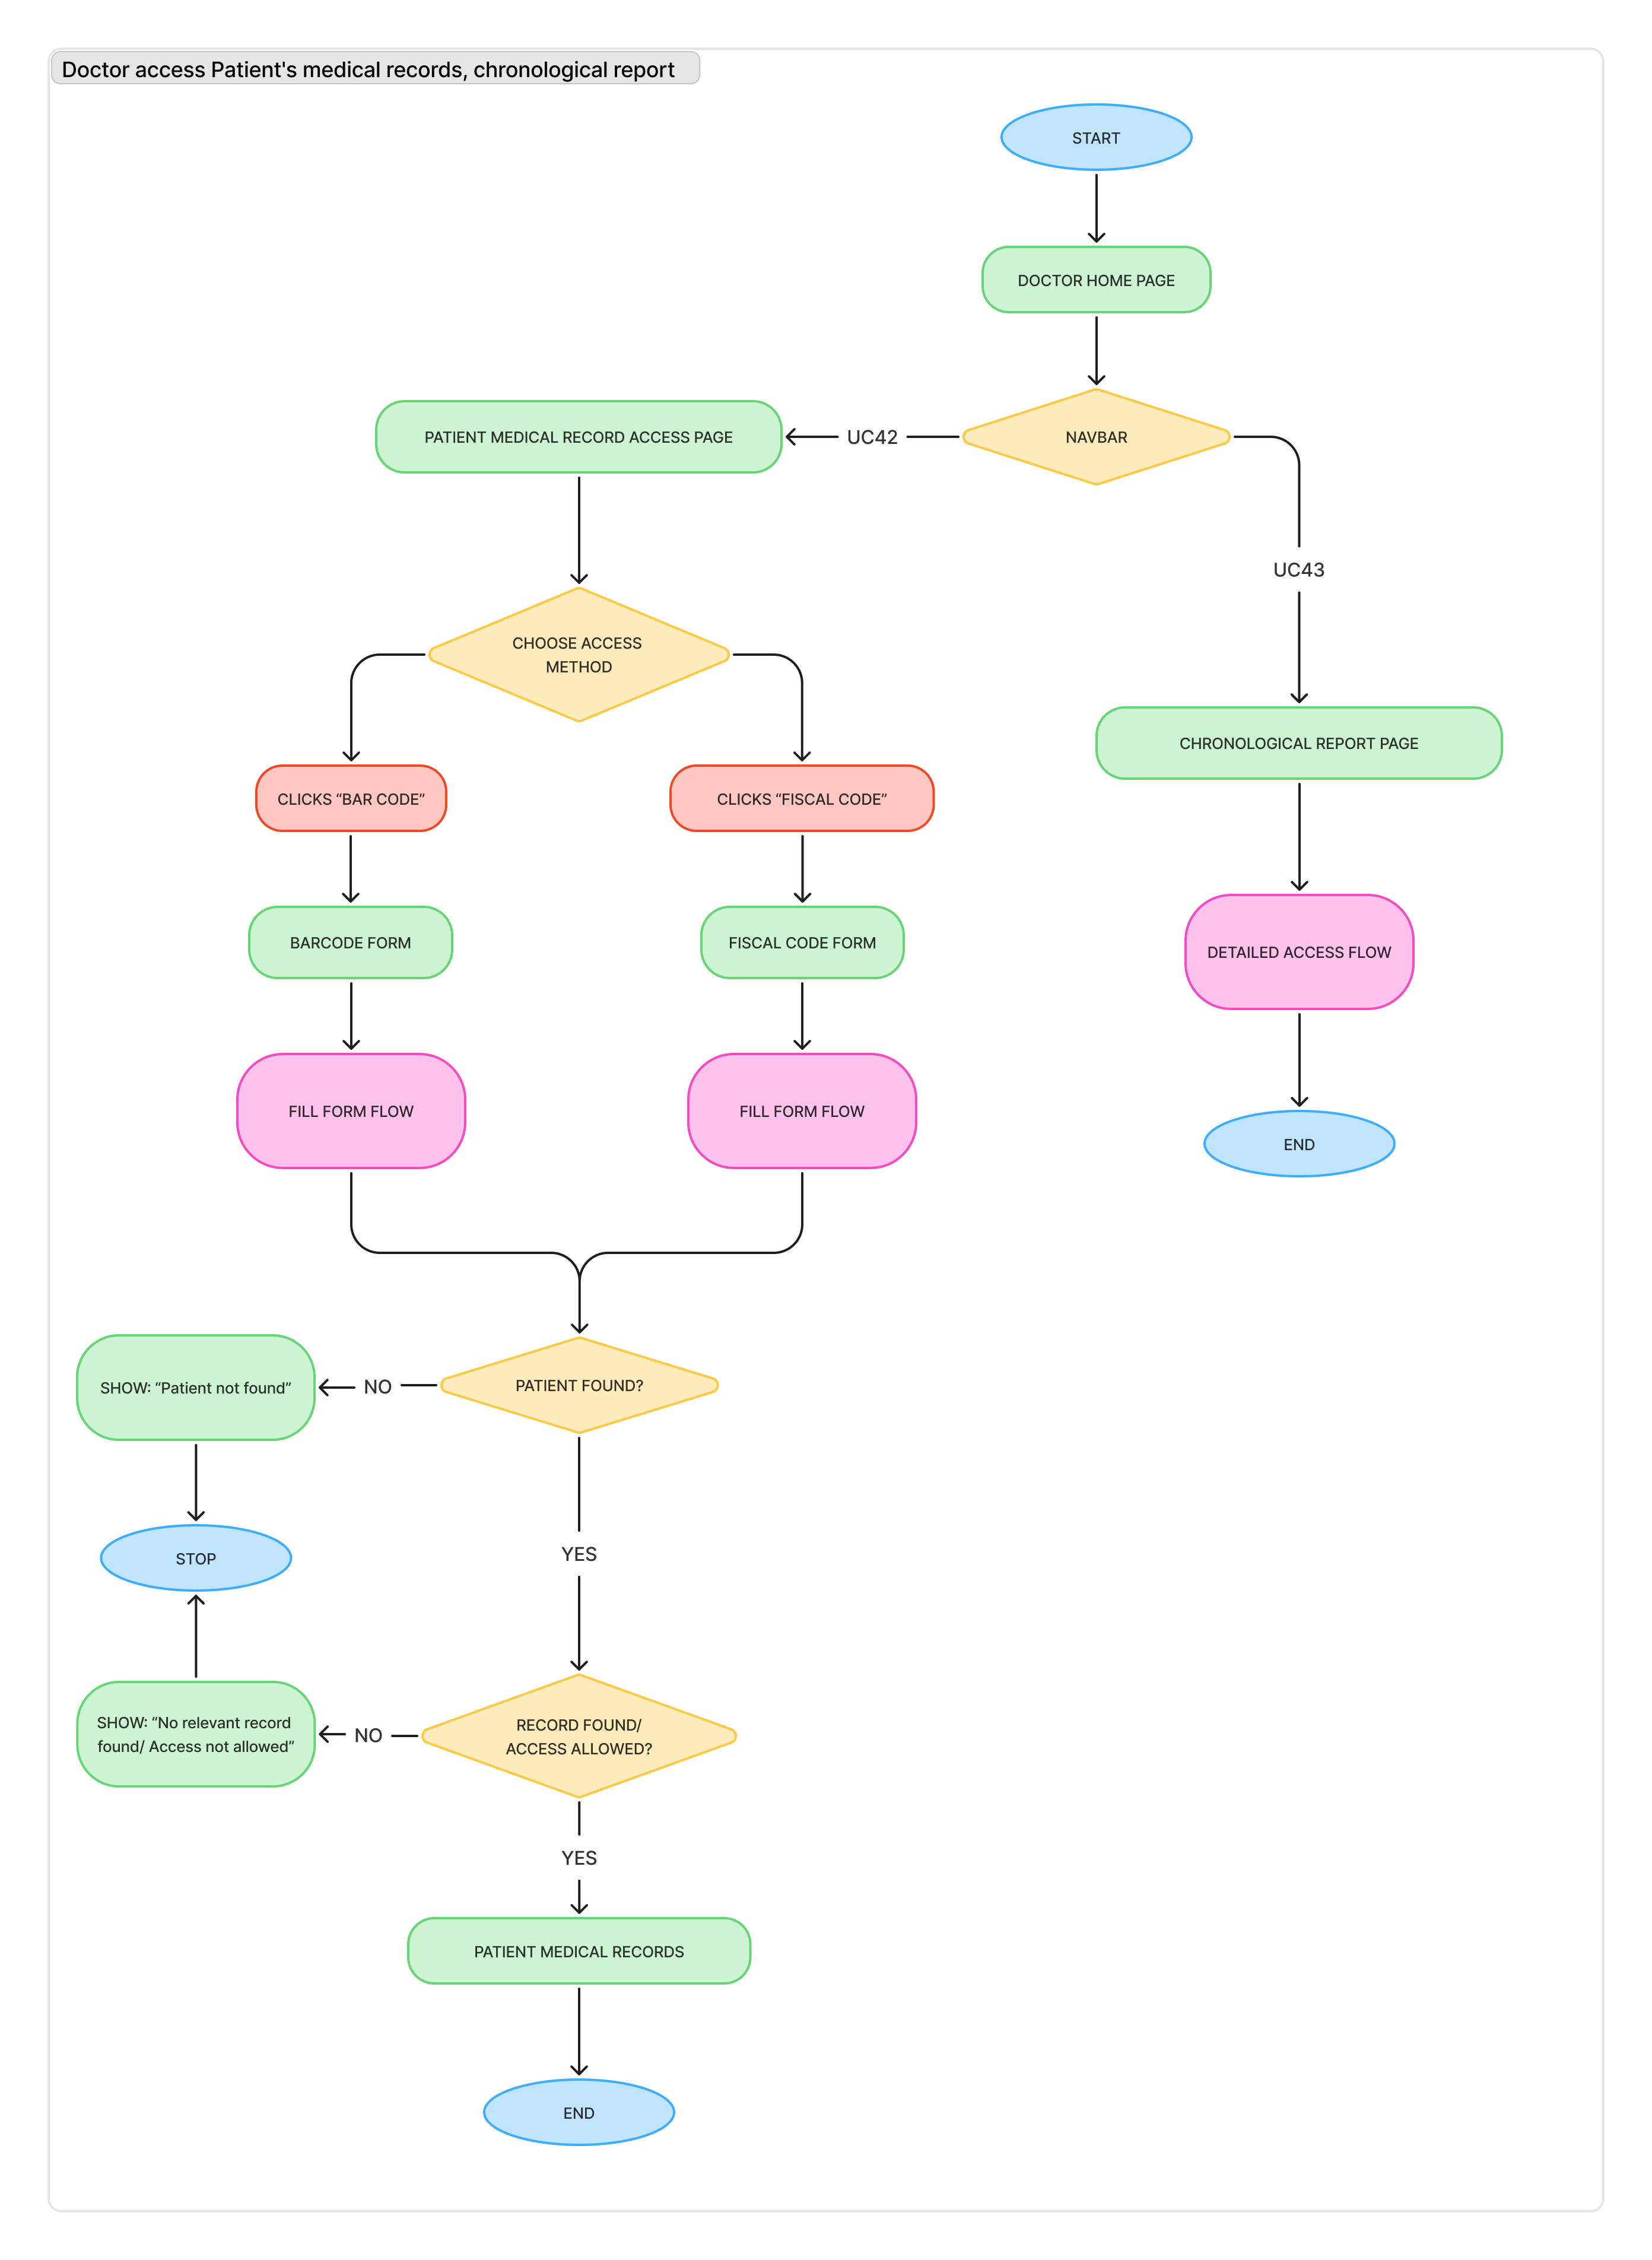
\includegraphics[width=0.7\textwidth]{User_Flows/DoctorMedicalRecordReport.png}
        \captionof{figure}{User flow regarding Doctor Access Patient's Medical Record, Chronological Report}
    \end{center}
    %\begin{itemize}   
    %\end{itemize}
\end{minipage}
\vspace{3em}

\begin{minipage}{\textwidth}
    \phantomsection
    \subsection{UF18. Doctor - Upload Prescriptions, Exemptions and Exam Results}
    The following user flow shows the steps a doctor takes to upload prescriptions, exemptions and exam results to a patient's profile. UC3 and UC4 are implemented.
    It refers to use cases \textbf{UC3, UC4}, and methods \textbf{Prescription.create(prescriptionData), Exemption.create(exemptionData), Examination.create(examinationData)} from the classes \textbf{Prescription, Exemption, Examination} of the class diagram.
    
    \begin{center}
        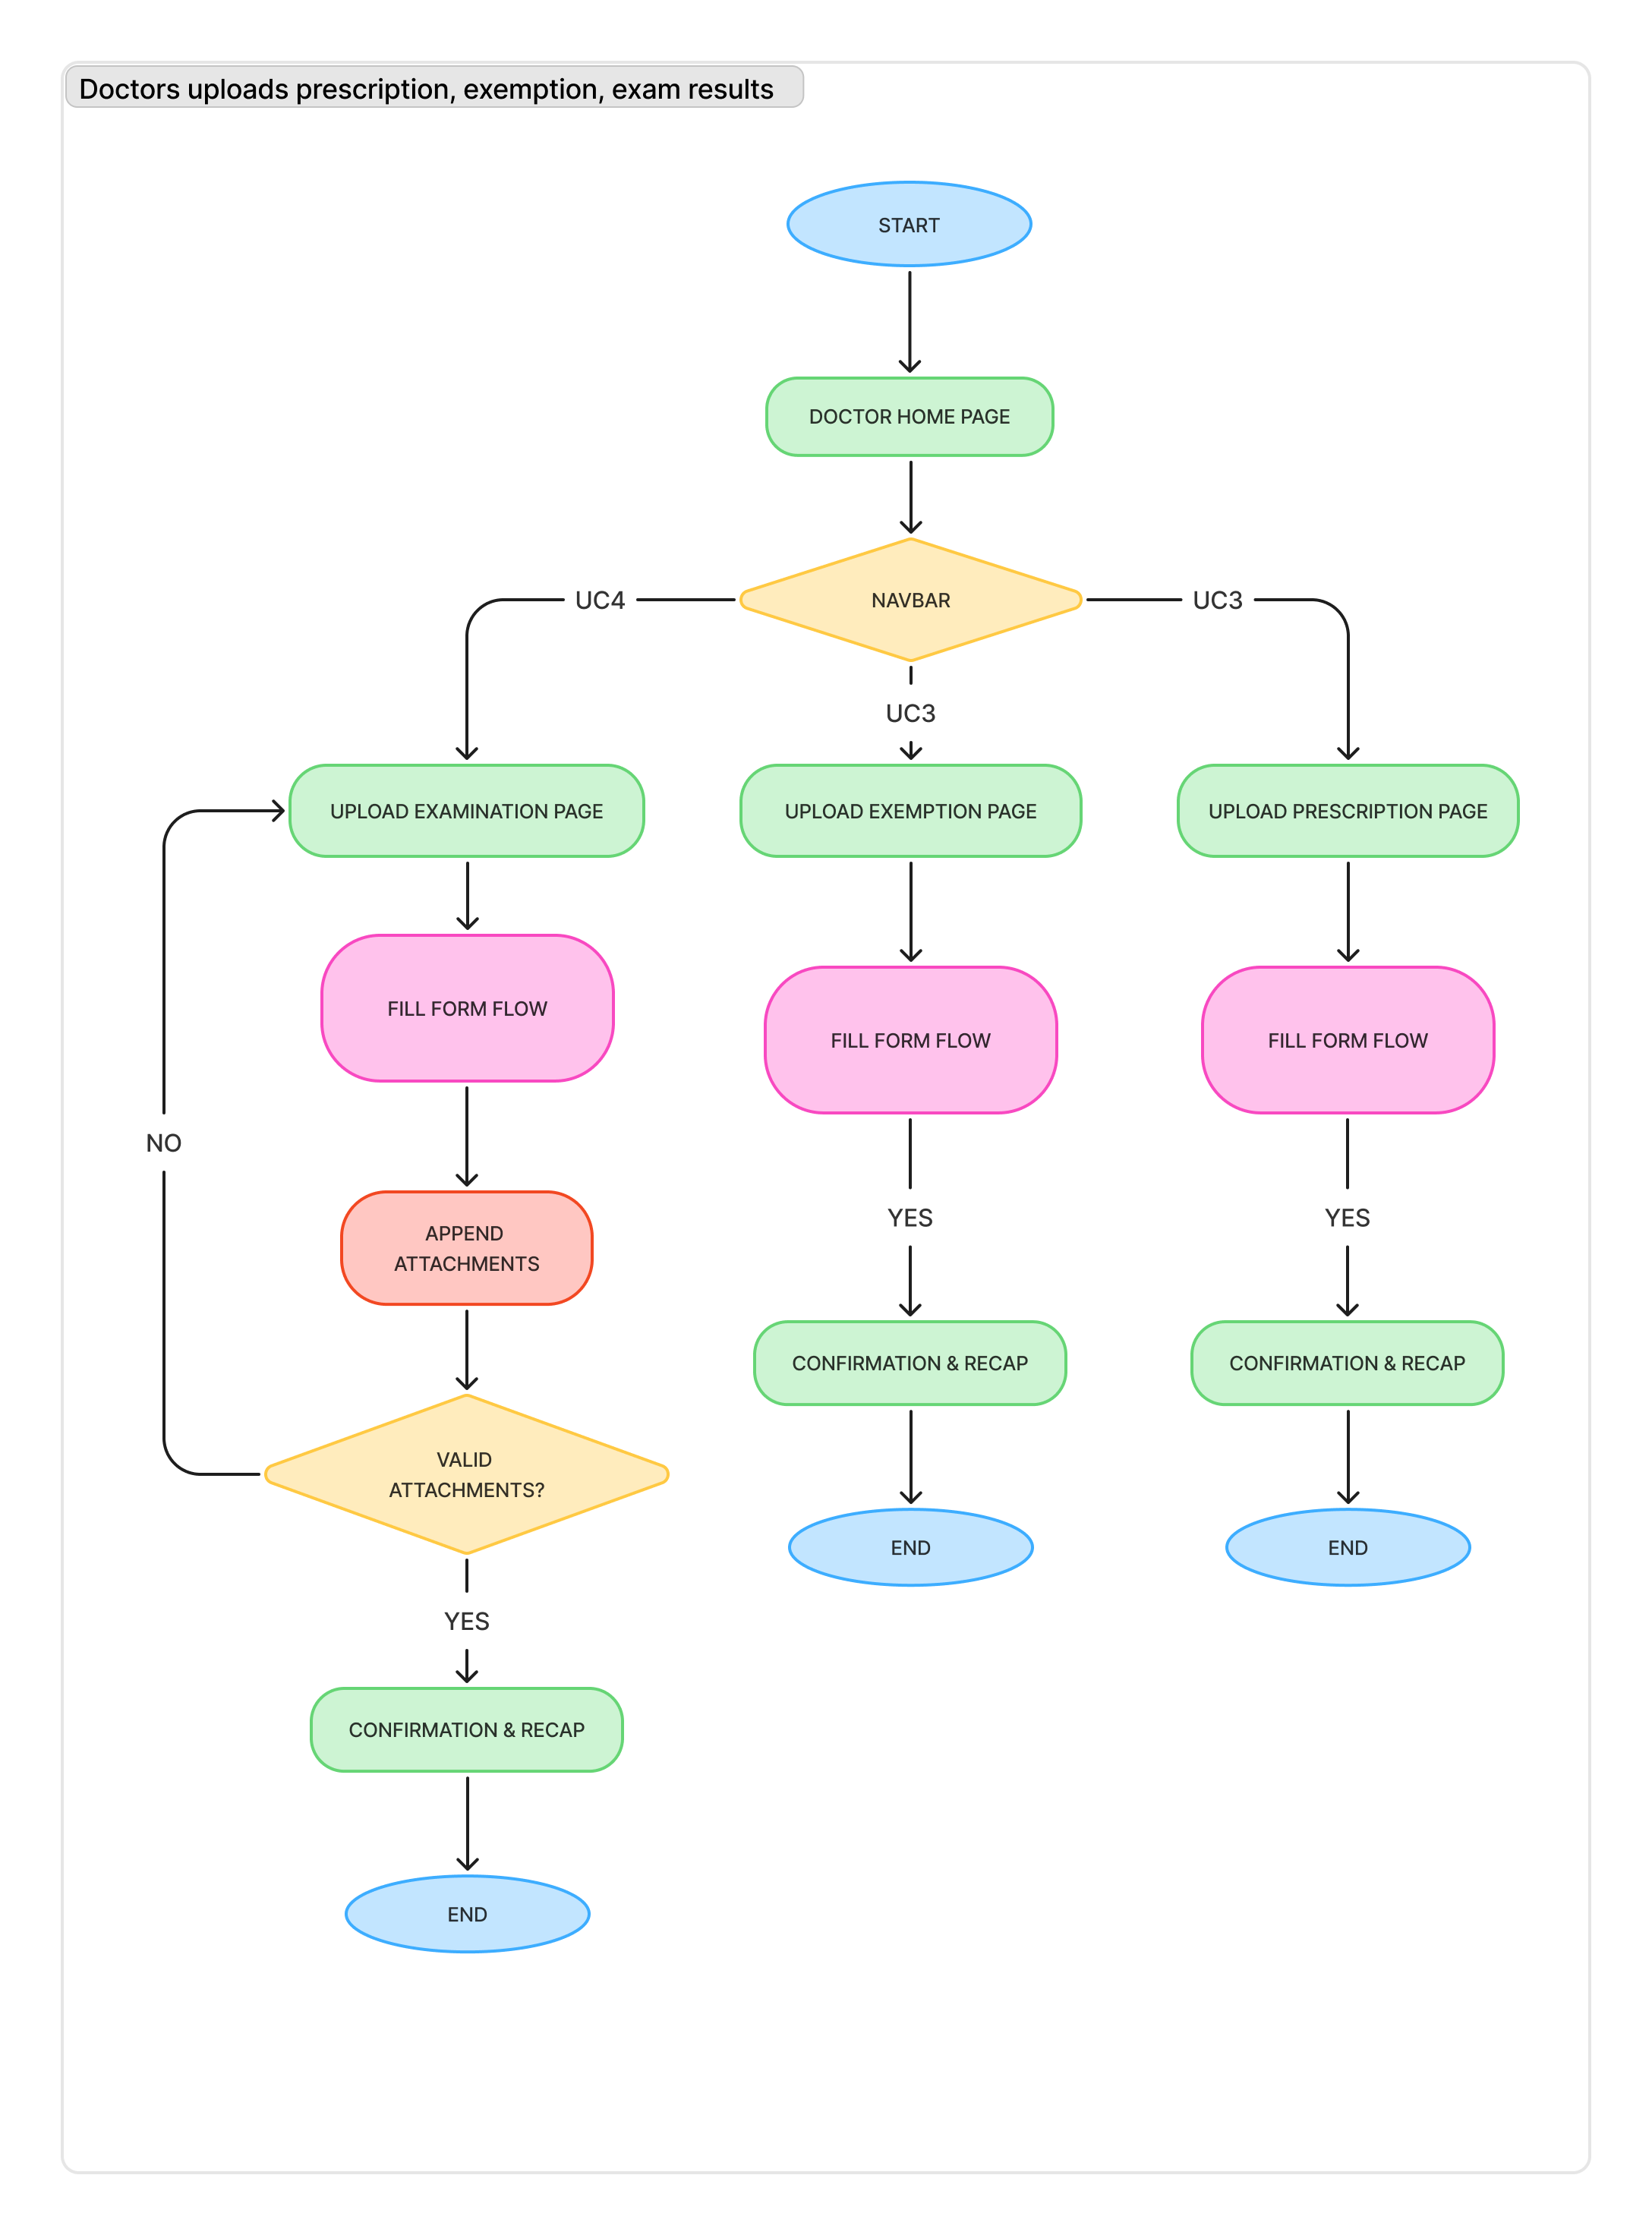
\includegraphics[width=0.9\textwidth]{User_Flows/DoctorUploads.png}
        \captionof{figure}{User flow regarding Doctor Upload Prescriptions, Exemptions and Exam Results}
    \end{center}
    %\begin{itemize}   
    %\end{itemize}
\end{minipage}
\vspace{3em}

\begin{minipage}{\textwidth}
    \phantomsection
    \subsection{UF19. Doctor - Cancel Appointment}
    The following user flow shows the steps a doctor takes to cancel one of their booked examinations. UC11 is implemented.
    It refers to use case \textbf{UC11}, and methods \textbf{cancel(reason : String)} from the class \textbf{Appointment} of the class diagram.
    
    \begin{center}
        
\includegraphics[width=0.8\textwidth,height=0.7\textheight,keepaspectratio]{User_Flows/DoctorAppointmentCancellation.png}
        \captionof{figure}{User flow regarding Doctor Appointment Cancellation}
    \end{center}
    %\begin{itemize}   
    %\end{itemize}
\end{minipage}
\vspace{3em}

\begin{minipage}{\textwidth}
    \phantomsection
    \subsection{UF20. Head of Department - Management Operations}
    The following user flow shows the steps a head of department takes to configure their department's services, capacity and doctor's workshifts. UC17, UC21 and UC44 are not implemented.
    It refers to use cases \textbf{UC17, UC21, UC44}, and methods \textbf{updateDepartmentTreatments(newTreatments), configureDepartmentCapacity(newCapacity),  setShiftPattern(Doctor, Shifts)} from the class \textbf{Head of Department} of the class diagram.
    
    \begin{center}
        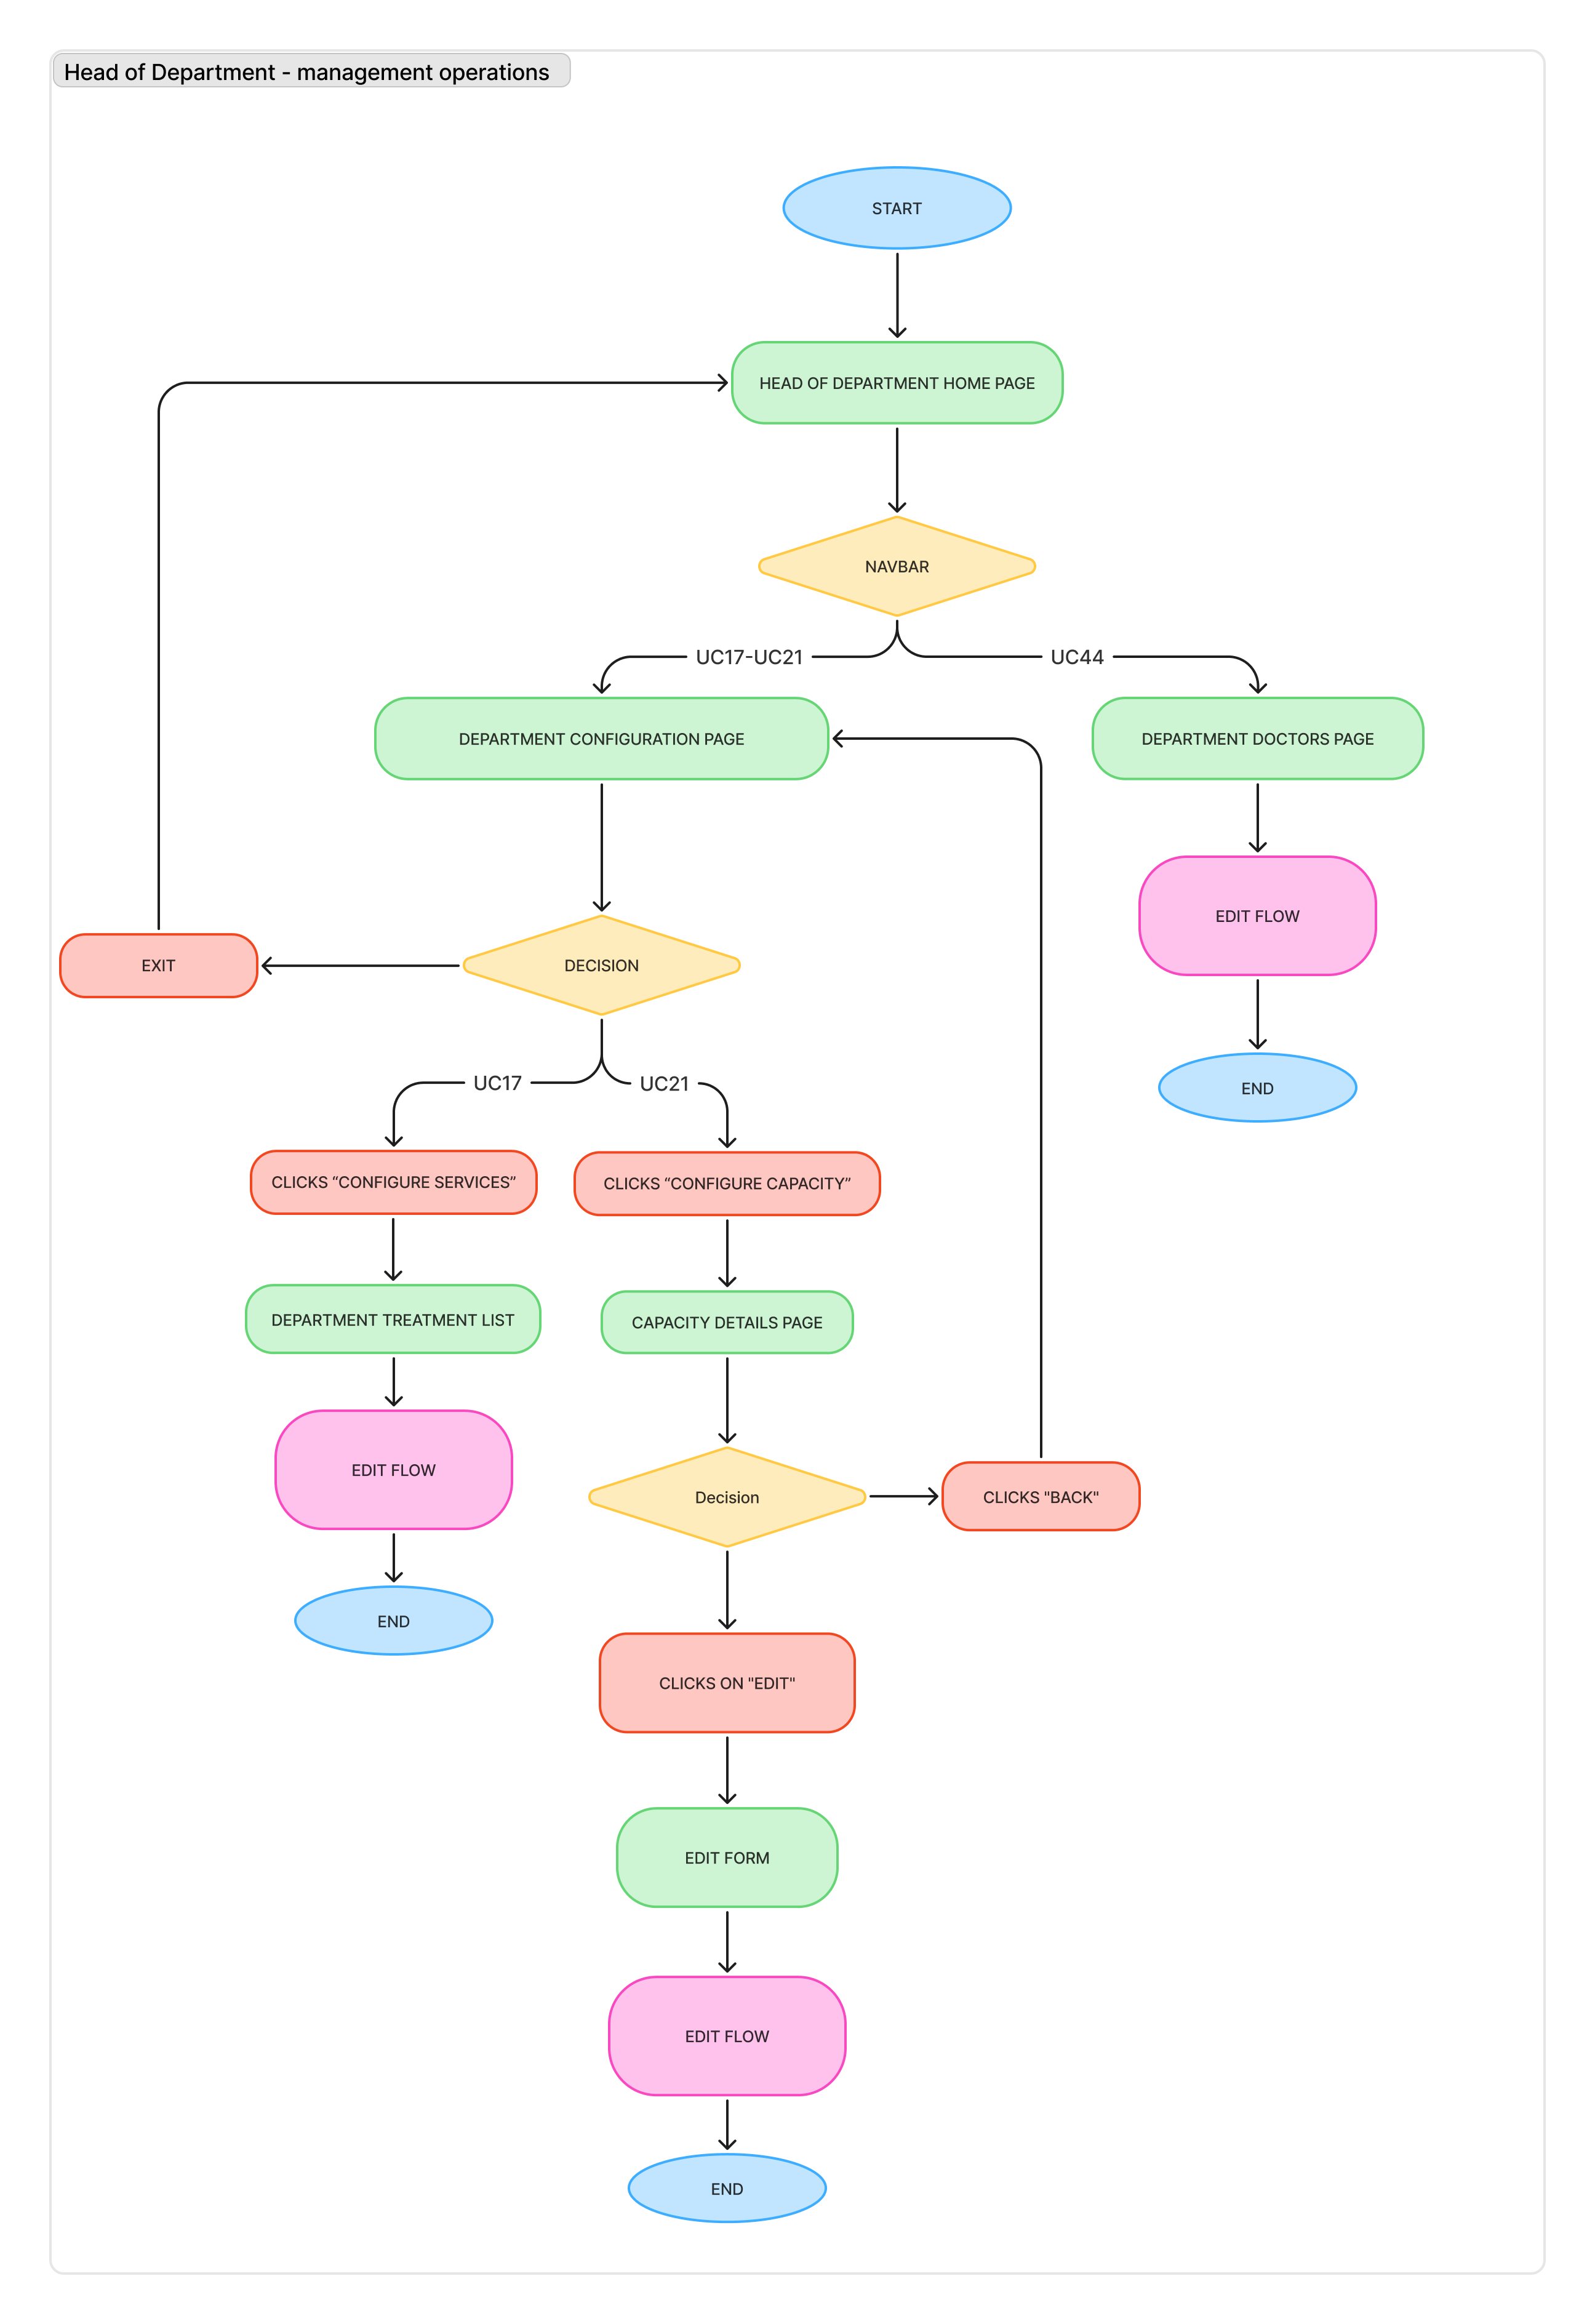
\includegraphics[width=0.8\textwidth]{User_Flows/DepartmentManagement.png}
        \captionof{figure}{User flow regarding Head of Department Management Operations}
    \end{center}
    %\begin{itemize}   
    %\end{itemize}
\end{minipage}
\vspace{3em}

\begin{minipage}{\textwidth}
    \phantomsection
    \subsection{UF21. Head of Department - Cancel Department Appointments}
    The following user flow shows the steps a head of department takes to cancel their department's booked appointments. UC11 is implemented.
    It refers to use case \textbf{UC11}, and methods \textbf{Appointment.cancel(reason)} from the class \textbf{Appointment} of the class diagram.

    \begin{center}
        
\includegraphics[width=0.9\textwidth, height=0.75\textheight, keepaspectratio]{User_Flows/DepartmentAppointmentCancellation.png}
        \captionof{figure}{User flow regarding Head of Department Cancel Department Appointments}
    \end{center}
    \end{minipage}
\vspace{3em}

\vspace{3em}

\begin{minipage}{\textwidth}
    \phantomsection
    \subsection{UF22. Head of Hospital - Insurances' Debt Management}
    The following user flow shows the steps a head of hospital takes to consult the insurances' debts owed to the hospital and register payments from insurance companies. UC18, UC19 and UC20 are not implemented.
    It refers to use cases \textbf{UC18, UC19, UC20}, and methods \textbf{Hospital.getInsuranceDebt(), OutstandingDebt.getHistory(), OutstandingDebt.settle(amount)} from the classes \textbf{Hospital, OutstandingDebt} of the class diagram.
    
    \begin{center}
        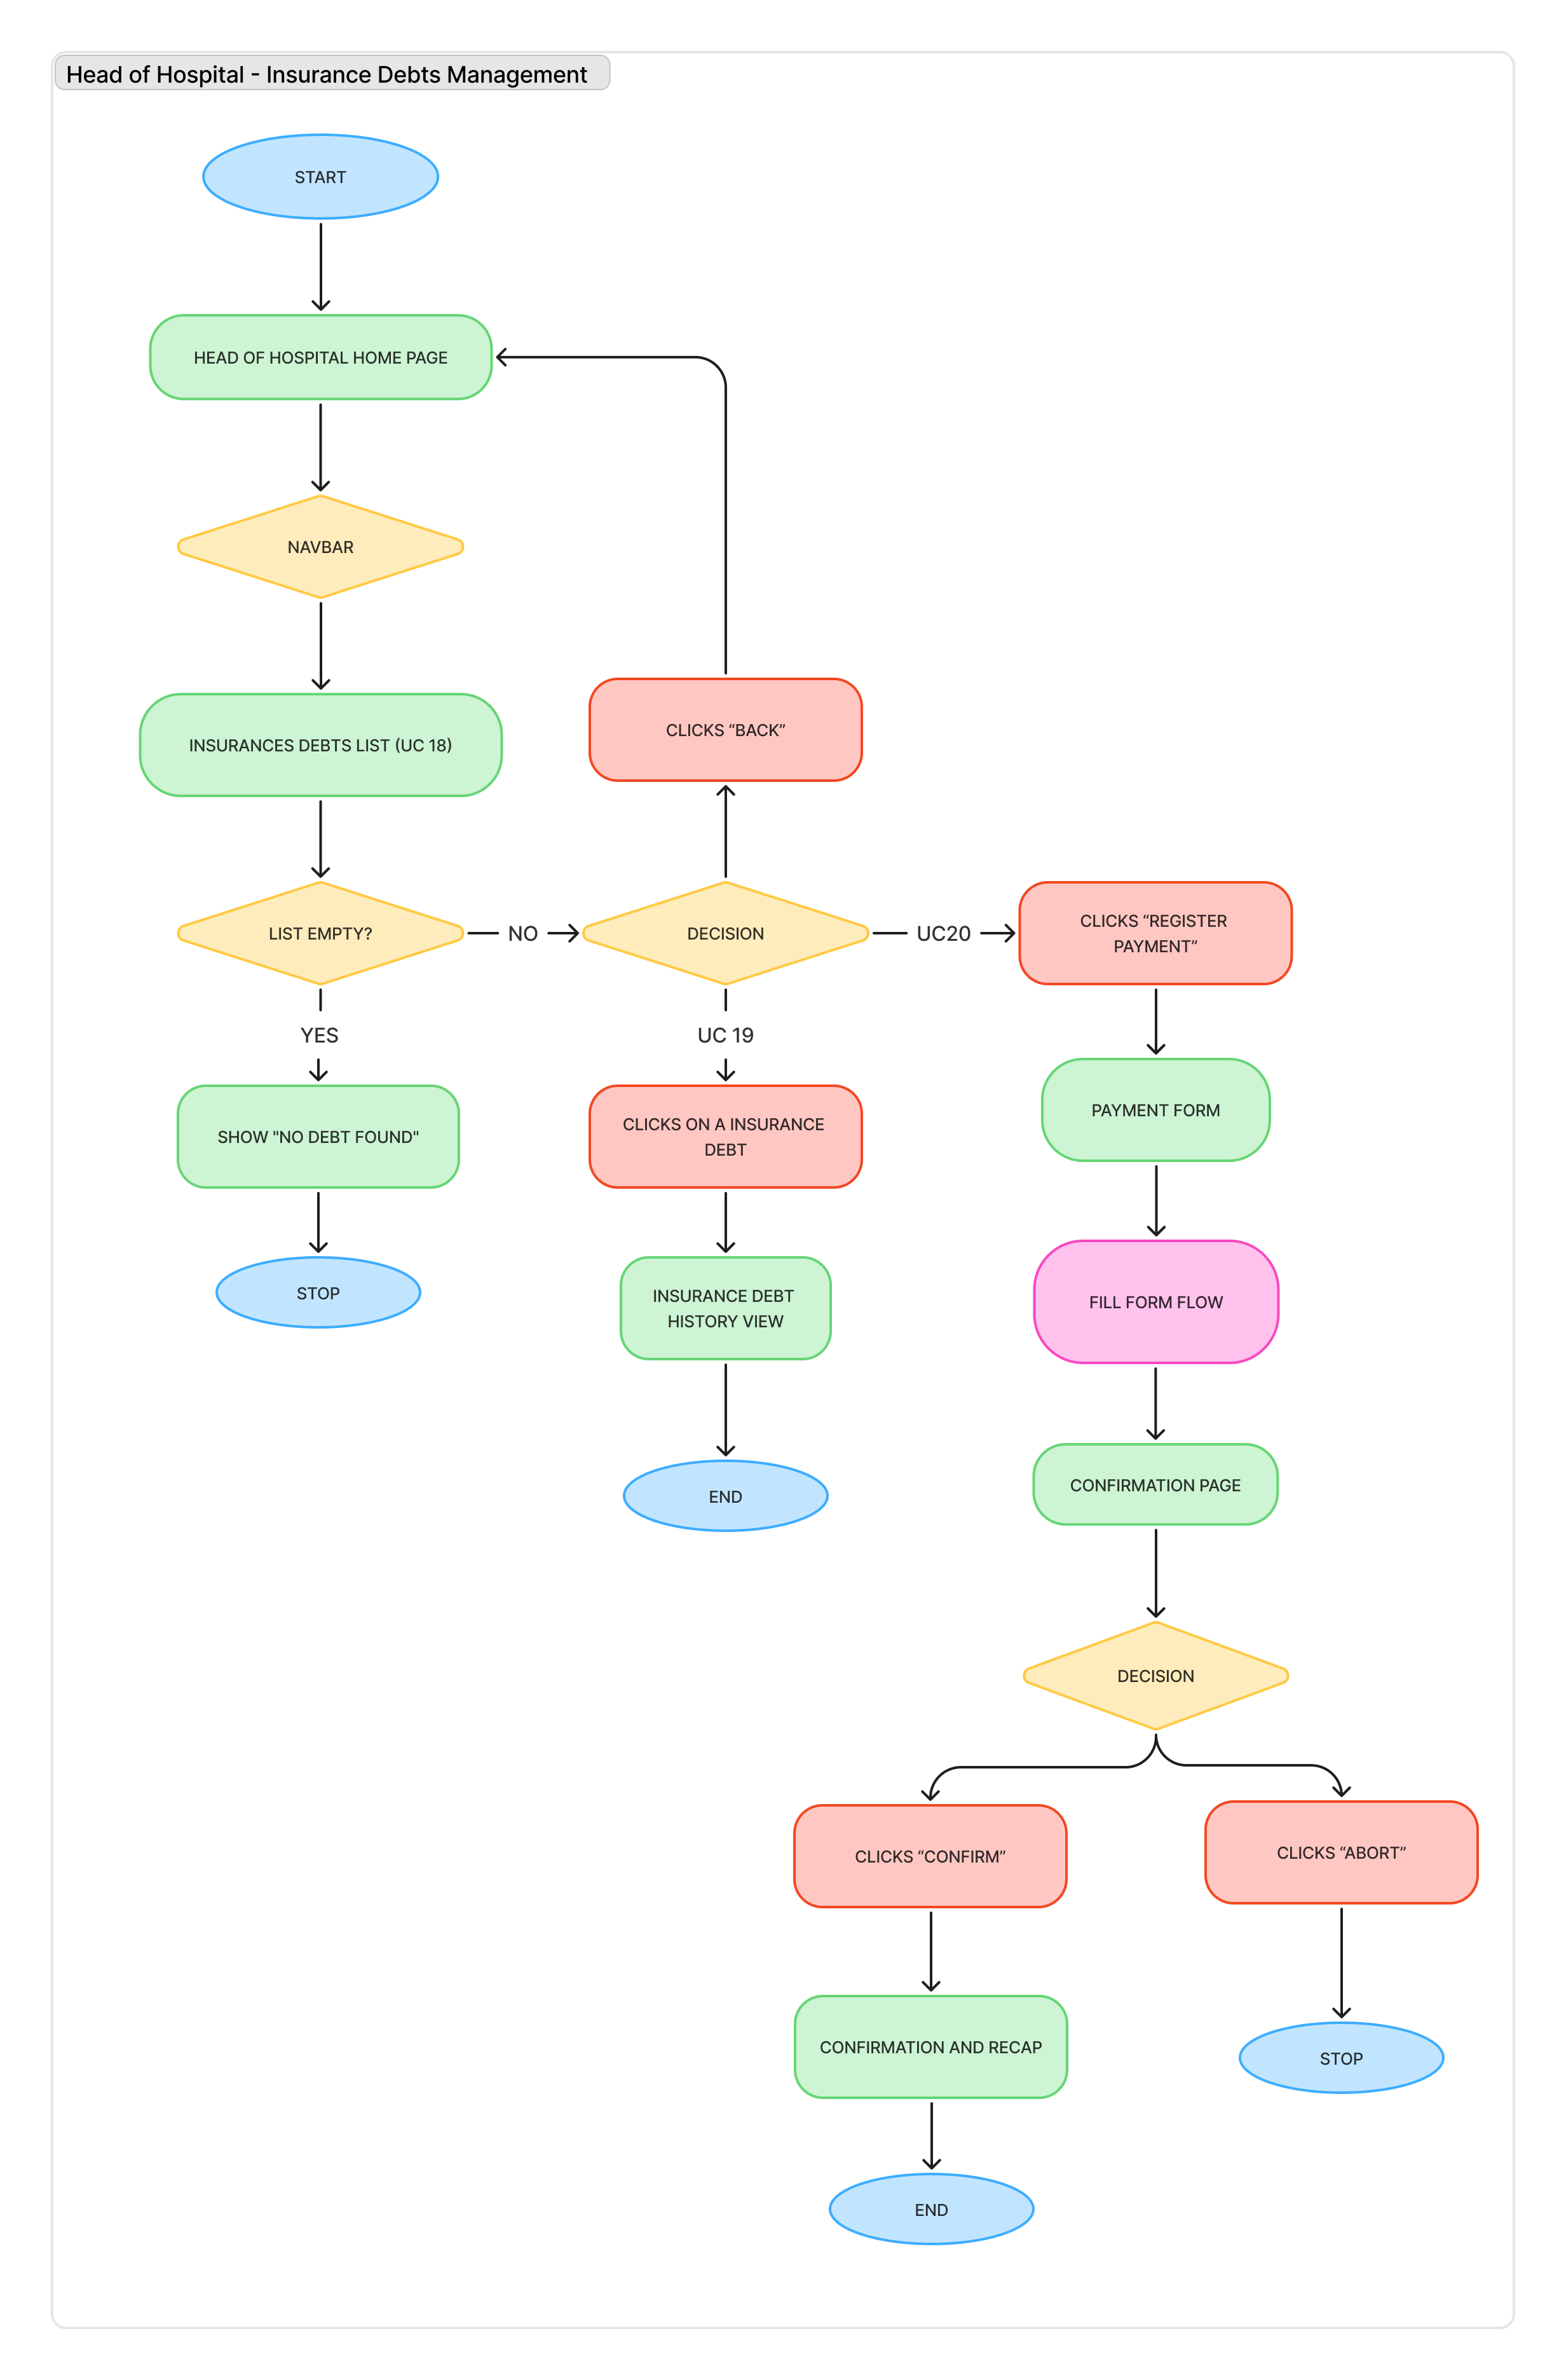
\includegraphics[width=0.8\textwidth]{User_Flows/HospitalDebtsManagement.png}
        \captionof{figure}{User flow regarding Head of Hospital Insurances' Debt Management}
    \end{center}    
    %\begin{itemize}   
    %\end{itemize}
\end{minipage}
\vspace{3em}

\begin{minipage}{\textwidth}
    \phantomsection
    \subsection{UF23. Head of Hospital - Department Assignments Management}
    The following user flow shows the steps a head of hospital takes to appoint a head of department and assign a doctor to a specific department. UC15 and UC16 are not implemented.
    It refers to use cases \textbf{UC15, UC16}, and methods \textbf{appointHeadOfDepartment(doctor, dept), allocateDoctors(doctors, dept)} from the class \textbf{Head of Hospital} of the class diagram.
    
    \begin{center}
        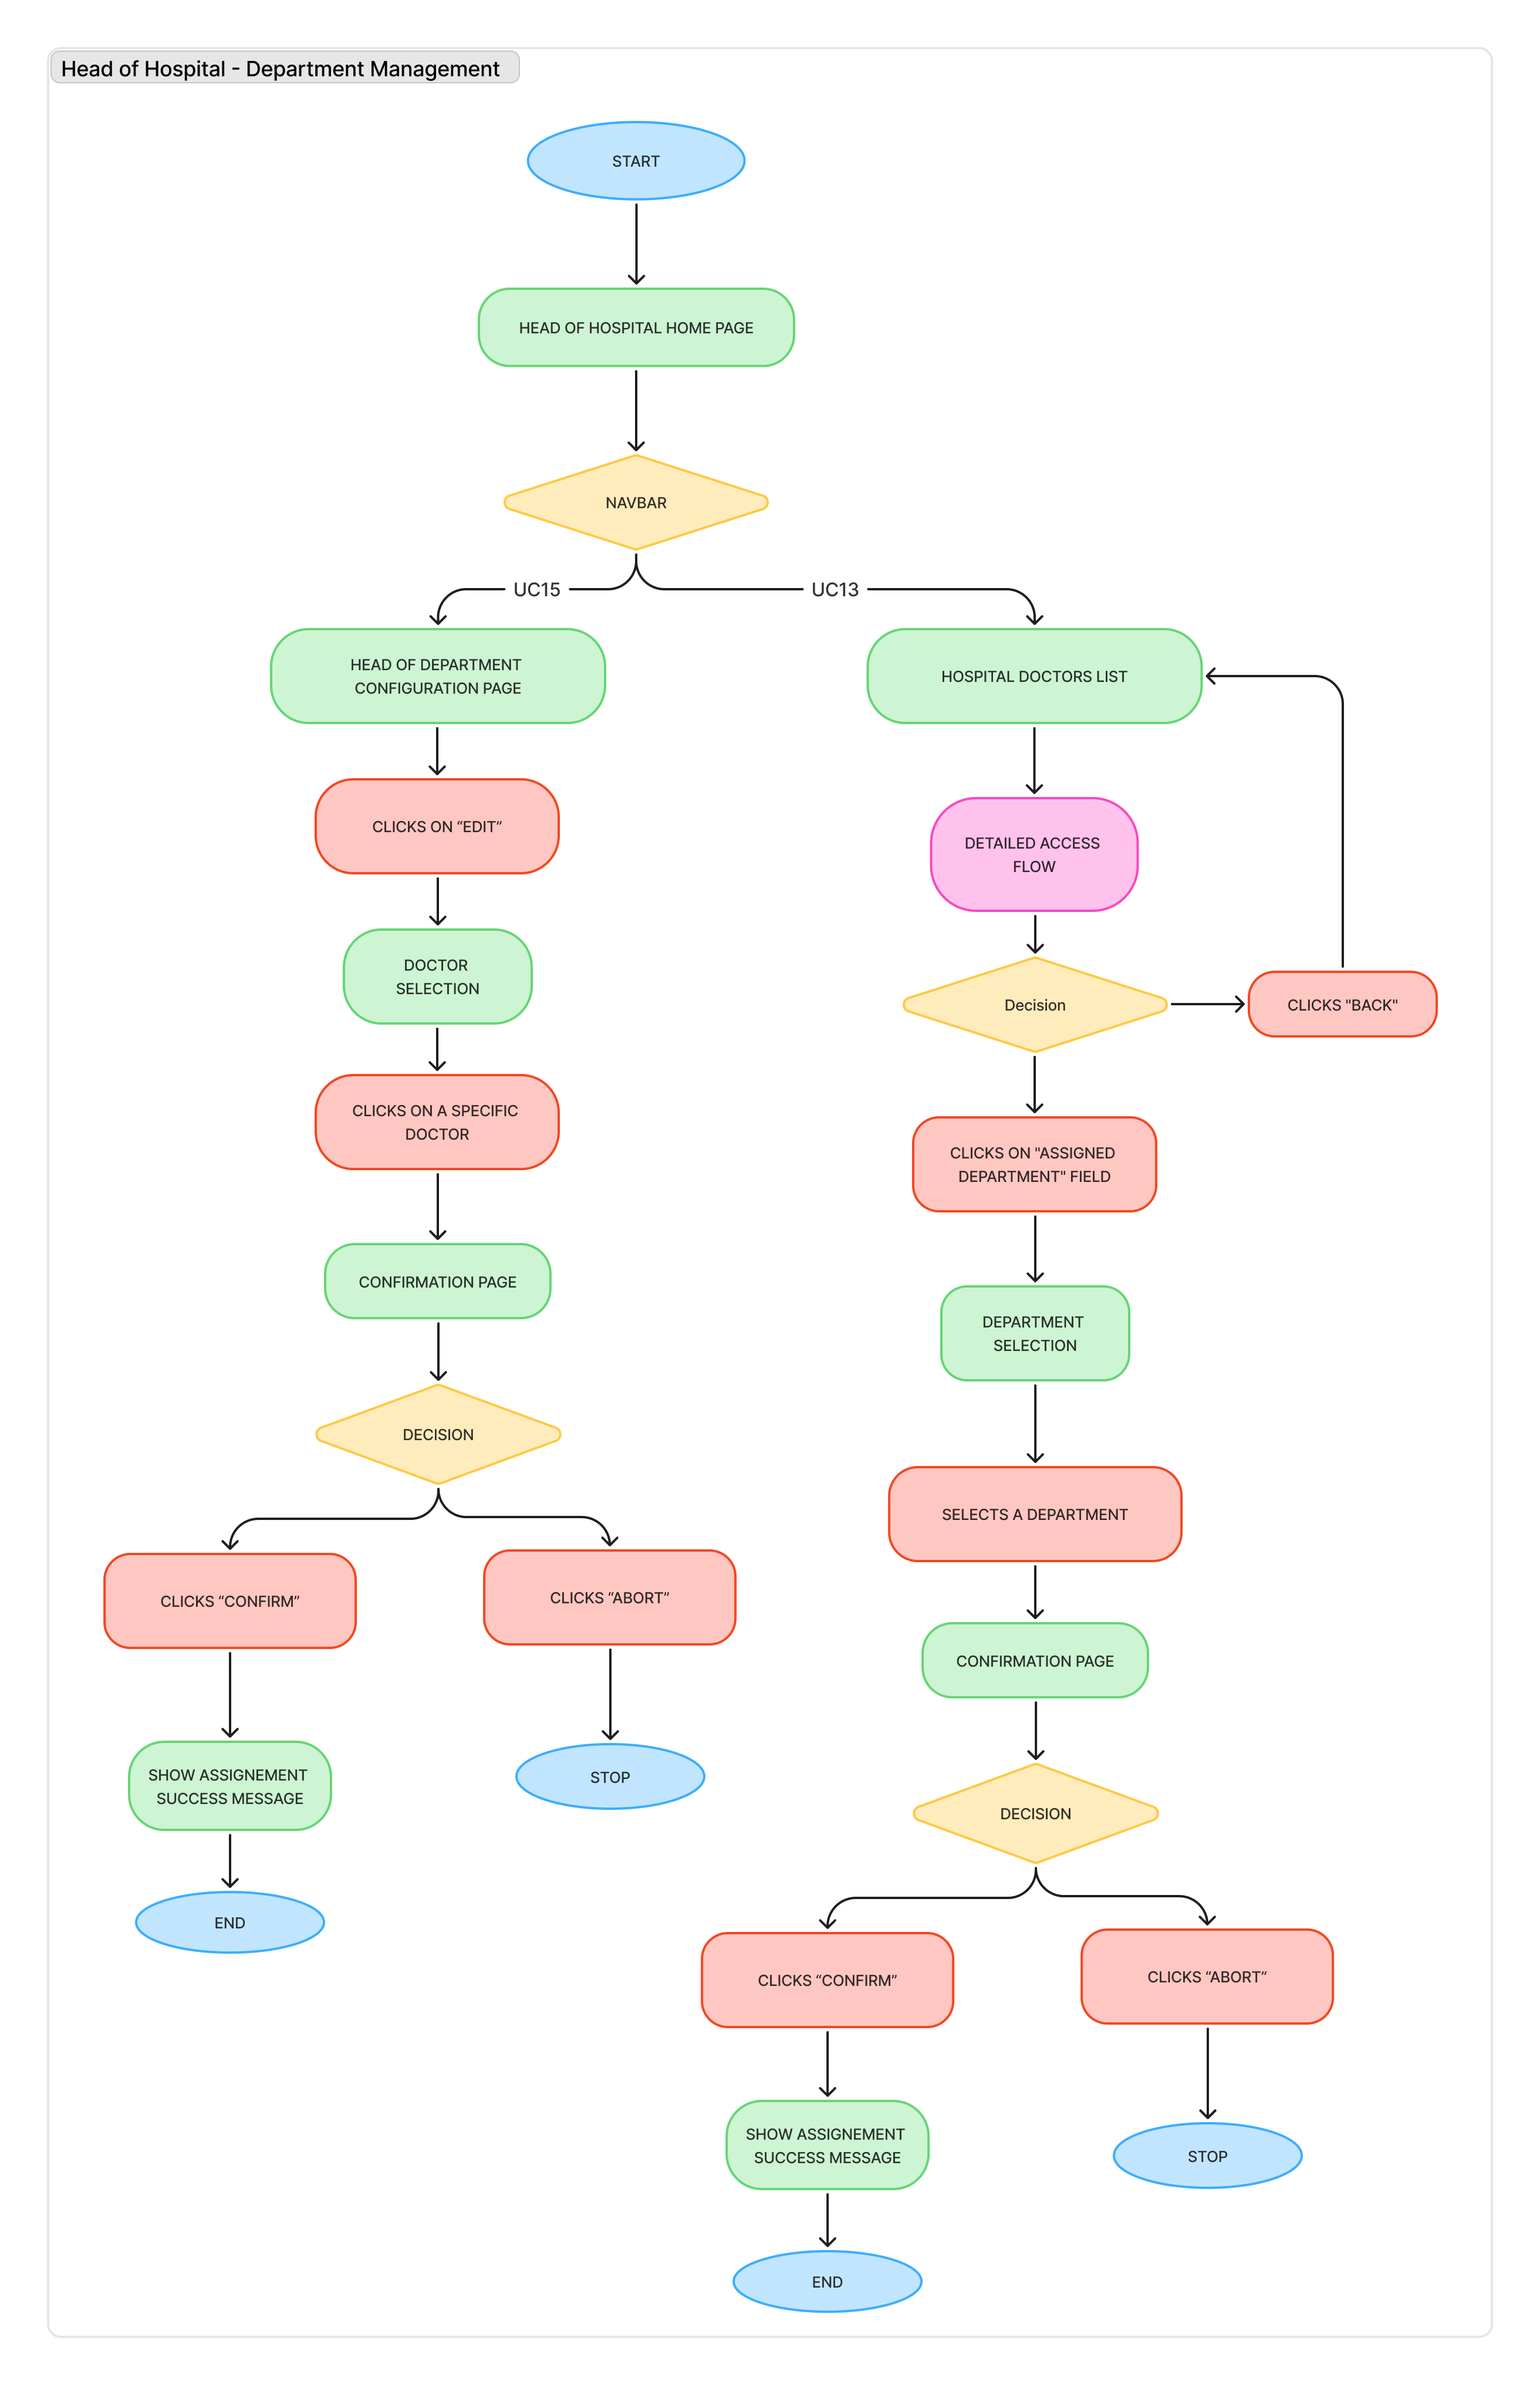
\includegraphics[width=0.7\textwidth]{User_Flows/HospitalHeadAssignements.png}
        \captionof{figure}{User flow regarding Head of Hospital Department Assignments Management}
    \end{center}
    %\begin{itemize}   
    %\end{itemize}
\end{minipage}
\vspace{3em}
